\section{Cloud Computing and Energy Efficiency Problem}
\label{sec:background}


% \subsection{Cloud computing}
\bx{Cloud computing is a computing model that offers a network of servers to their clients in a on-demand fashion.} From NIST's definition \cite{Mell:2011jj}, \textit{"cloud computing is a model for enabling ubiquitous, convenient, on-demand network access to a shared pool of configurable computing resources (e.g., networks, servers, storage, applications and services) that can be rapidly provisioned and released with minimal management effort or service provider interaction."} Hence, Cloud computing has major functionalities for providing facilities to cloud users.

\begin{figure}
	\centering
	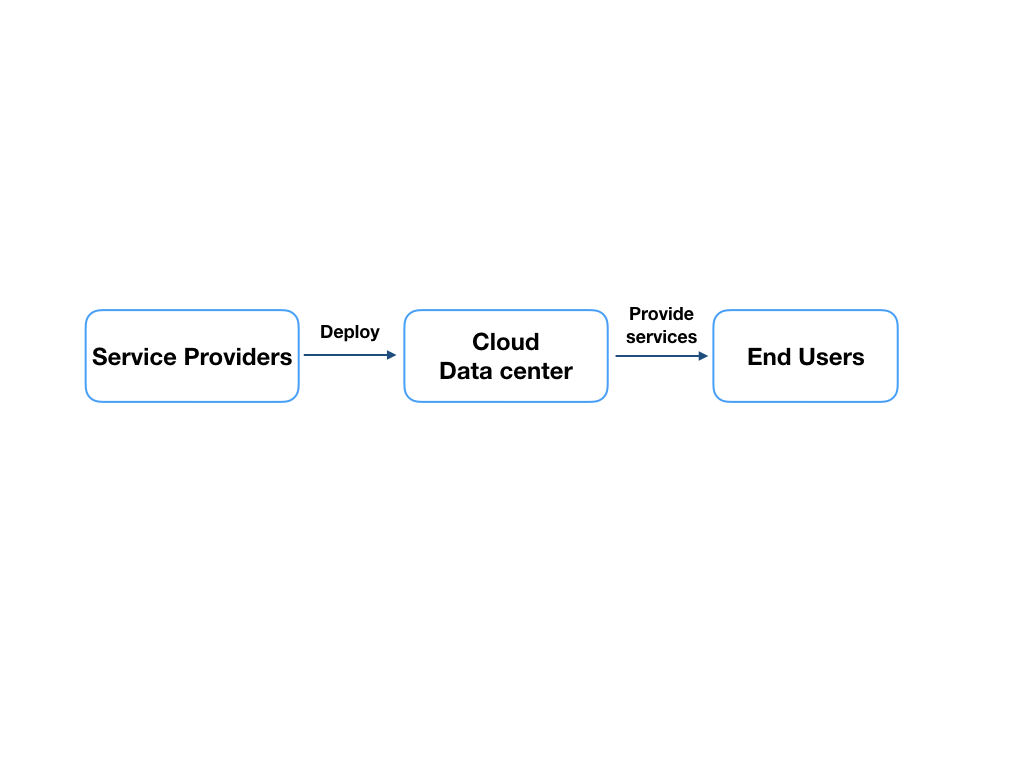
\includegraphics[width=0.6\textwidth]{pics/stakeholders.png}
	\caption{Stakeholders of Cloud computing \cite{Jennings:2015ht}}
	\label{fig:stakeholders}
\end{figure}

\bx{To give an example of how Cloud computing works (see Figure \ref{fig:stakeholders}), consider the case:} a \emph{Cloud provider} builds a data center containing thousands of servers. These servers connect with a network. 
% These servers are virtualized which means they are partitioned into smaller units of resources called \emph{Virtual Machines (VMs)} or \emph{Containers} \cite{Felter:2015ki}. 
To use these remote servers, \emph{Cloud user} (e.g an application provider), can deploy and access their applications (e.g Endnote, Google Drive and etc.) in these servers from anywhere in the world. Once the applications start serving, \emph{End users} can use them without installing on their local computers. Cloud providers charge fees from Cloud users for infrastructure. Cloud users charge fees from End users for using applications. \tran{Therefore, from cloud providers' perspective, both accommodating more applications and reducing energy consumption lead to the increase of profit.}

\bx{The major expense of a cloud provider is energy consumption \cite{Kaplan:up01fR-k} and physical machines (PMs) (e.g servers) contribute to a majority of the energy.} As shown in Figure \ref{fig:consumption}, both the cooling system and physical machines (PMs) account for 40\% of energy. However, PMs' energy efficiency are low on average  \cite{Hameed:2016cmb}.
The reason for low energy efficiency is the disproportion between the utilization of PMs and the energy consumption of PMs. \howto{For example, when CPU utilization of a PM is 15\%, the energy consumption of the PM is 70\% of its peak time.} Therefore, 
cloud providers can reduce the energy consumption by improving the utilization of PMs.

% \tran{In order to solve the problem, a concept of
% \emph{energy proportional computing} \cite{Barroso:2007jt} raised to address the disproportionate between utilization and energy consumption by using virtualization technology.}

\tran{In order to solve the low energy efficiency caused by low utilization of PMs, cloud providers use a resource management system to manage the applications.}

\begin{figure}
	\centering
	% \begin{subfigure}[b]{0.45\textwidth}
		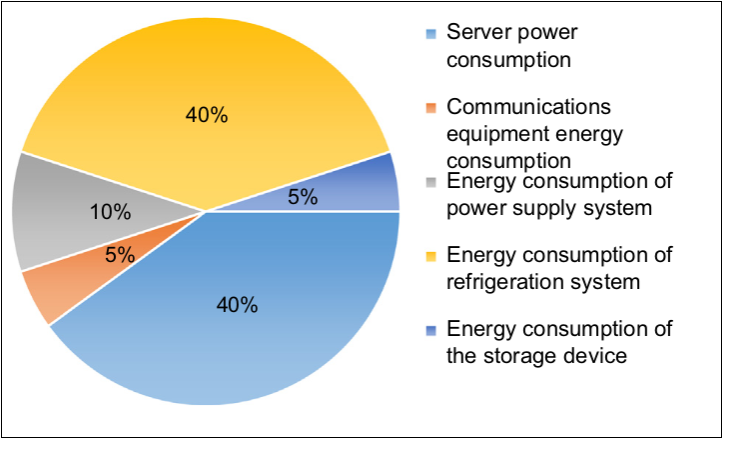
\includegraphics[width=0.35\textwidth]{pics/energyConsumption.png}
		\caption{Energy consumption distribution of data centers \cite{Rong:2016js}}
		\label{fig:consumption}
	% \end{subfigure}
	% \begin{subfigure}[b]{0.45\textwidth}
	% 	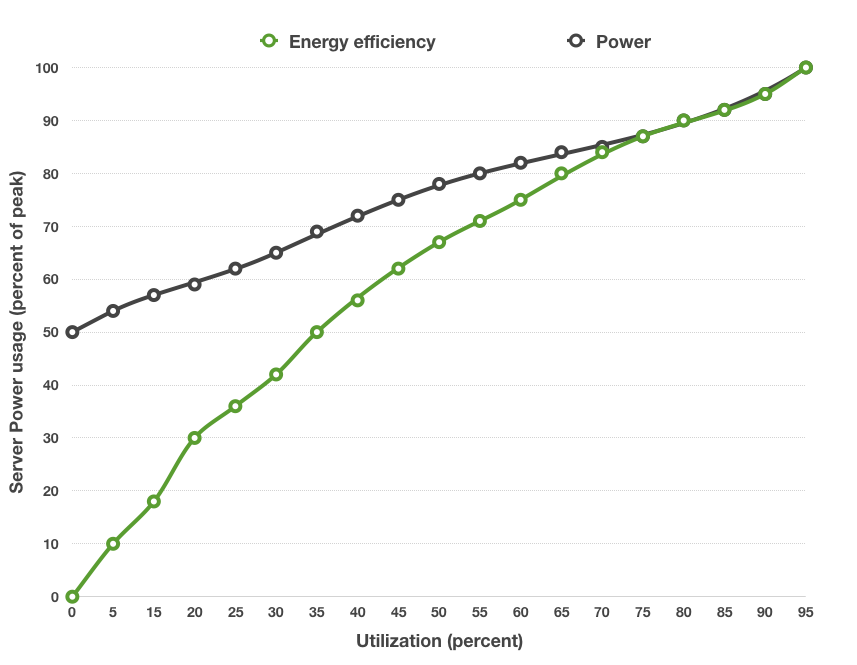
\includegraphics[width=\textwidth]{pics/util.png}
	% 	\caption{Disproportionate between utilization and energy consumption \cite{Barroso:2007jt}}
	% 	\label{fig:unproportional}
	% \end{subfigure}
\end{figure} 

\section{Cloud Resource Management}
\label{sec:resource_management}
\bx{Cloud resource management is a process of allocating computation resources (e.g CPU and memory) to Cloud users to run their applications. Meanwhile, resource management aims to achieve low energy consumption in cloud} \cite{Jennings:2015ht}.

Resource management applies two types of virtualization: virtual machine (VM) and container on four management steps (see Section \ref{sec:statement}): collecting PMs' utilization data, analyzing available PMs, deciding the placement of applications, and executing the placement. Furthermore, in the third step of placement decision, resource management has three common scenarios: initial placement, periodic placement, and dynamic placement. Resource management uses distinct server consolidation strategies on these placement scenarios based on different virtualiazation technologies to achieve energy efficiency. 

This section will first introduce and compare two types of virtualization: VM-based and container-based and then illustrate 
three placement decision scenarios. 

\subsection{Virtualization Technologies}
\label{sec:virtualization}
% \bx{Two technologies can be used to achieve server consolidation: clustering and virtualization.} Clustering is used in a situation that the applications running in bare-mental PMs are I/O intensive. This is because current virtualization technologies  such as KVM \cite{Kivity:2007wu} or Xen \cite{Barham:2003cj} are not suitable for data intensive application because they have a 20\% to 55\% of reduction of I/O bandwidth (e.g disk reads and writes, network bandwidth) in comparison with bare-mental PM \cite{Shafer:2010vh}. In our research, we consider the applications which require small CPU utilization (e.g 15\%) and low I/O needs such as web services, therefore, this section mainly discusses the virtualization technology.

\bx{Resource management uses virtualization technologies \cite{Uhlig:2005do} to achieve a finer granularity management than the traditional way.} In comparison with traditional management -- allocating an application to a PM -- virtualized management partitions PM's resources (e.g. CPU, memory and disk) into several independent units and allocates applications into these units. 
The most common units are virtual machines (VMs) and containers.

Virtualization technology rooted back in the 1960s' was originally invented to enable isolated software testing. Because VMs can provide good isolation for applications running without interfering with each other \cite{Somani:2009ho}. Soon, people realized that virtualization can improve the utilization of hardware resources: with each application deployed in a VM, a PM can run multiple applications. 

The next two sections illustrate two classes of virtualization (see Figure \ref{fig:comparison}): VM-based and container-based virtualization and then compares the two virtualizations.

\begin{figure}
	\centering
	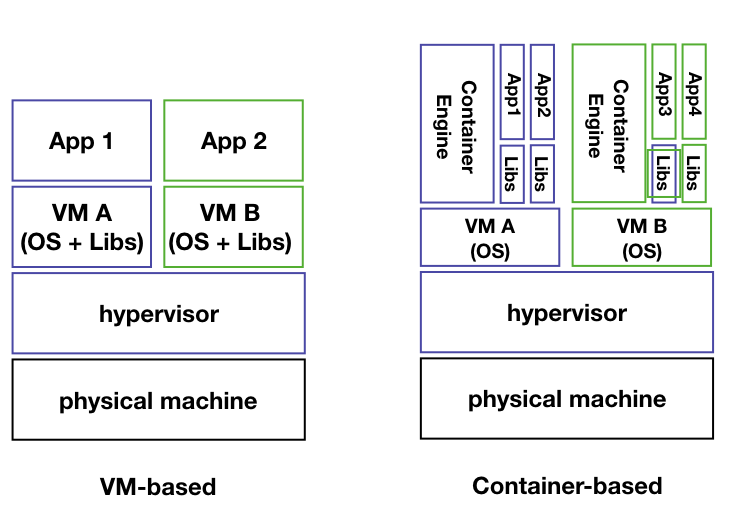
\includegraphics[width=0.7\textwidth]{pics/comparison.png}
	\caption{A comparison between VM-based and Container-based virtualization \cite{Piraghaj:2016bw}}
	\label{fig:comparison}
\end{figure}

\subsubsection{VM-based Virtualization} 

\bx{A VM-based virtualization has three-layers of structure: PM-Hypervisor-VM (see Figure \ref{fig:comparison} left-hand side).} 
The hypervisor or the virtual machine monitor (VMM) is a software layer on top of PM. A hypervisor arbitrates accesses to the PM's resources so that VMs can share resources on the PM. Some implementations of VM-based hypervisors such as Xen \cite{Barham:2003cj}, KVM \cite{Kivity:2007wu}, and VMware ESX \cite{Waldspurger:2002db} dominate this field in recent years. On of top of hypervisor, \textbf{VMs} are the fundamental resource management units. A VM allows independent Operating System (OS) to run on it.  

In addition, hypervisors support dynamic migration techniques (e.g pre-copy \cite{Clark:2005ud} and post-copy \cite{Hines:2009fv}) that can move VMs from one PM to another. Therefore, resource management can improve the utilization of a PM by migrating VMs to that PM.

% \bx{VMs can be used to reduce the energy consumption in data centers by utilizing the technology of live migration.} live migration  \cite{Hines:2009fv} can move a VM from one PM to another without interrupting the application running inside the VM. A common practice gathers several low utilized VMs into a PM so that the utilization of the PM is improved and idle PMs are turned off to save energy. This practice is called server consolidation which will be discussed in Section \ref{consolidation}.

\subsubsection{Container-based Virtualization} 
% It allows applications to have their own separated development environment such as libraries. 

\begin{figure}
	\centering
	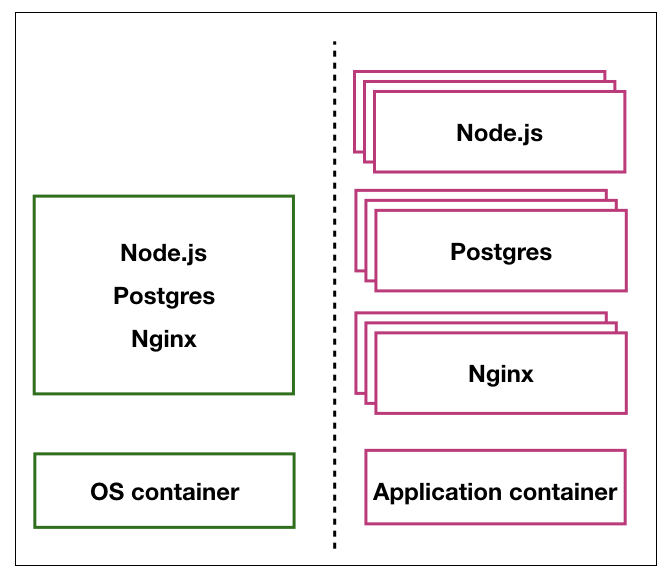
\includegraphics[width=0.4\textwidth]{pics/container_OS_APP.png}
	\caption{A comparison between OS container and Application container \cite{Piraghaj:2017vi}}
	\label{fig:comparison_container}
\end{figure}

\bx{A Container-based virtualization has four-layers of structure: PM-Hypervisor-VM-Container (see Figure \ref{fig:comparison} right-hand side).} Container-based virtualization is also addressed as operating-system-level virtualization because containers run on top of VMs. Specifically, container-based virtuliazation includes two classes: OS container and application container \cite{Piraghaj:2017vi}. 

\bx{OS containers (Figure \ref{fig:comparison_container} left-hand side) have a one-on-one relationship with VM.}
Multiple applications run inside an OS container. Three implementations of OS-level of containers: OpenVZ, Google's control groups, and namespace \cite{Rosen:2013wt} are widely used in Google and Facebook.

\bx{Application containers (Figure \ref{fig:comparison_container} right-hand side) have a many-to-one relationship with VM.} A single application runs on an application container. Major implementations such as Docker, Rocket and Kubernetes \cite{Bernstein:2014ur} are very popular in the software industry. 

\bx{In comparison with OS container, an application container is much more flexible because each container has its separated environment (e.g. libraries) for applications.} Furthermore, application containers provide a finer granularity of resource management by enabling an application level of operations including deployment, scaling, and migration.  

Notice that, in the following content, we use ``container'' to represent ``application container''. 
We do not discuss Os container because it is very similar to a VM.

% He et al \cite{He:2012im} propose an hierarchical resource management architecture for application container (see Figure \ref{fig:container_architecture}). The major functionality of Cloud controller is to provide a global optimization.

% \begin{figure}
% 	\centering
% 	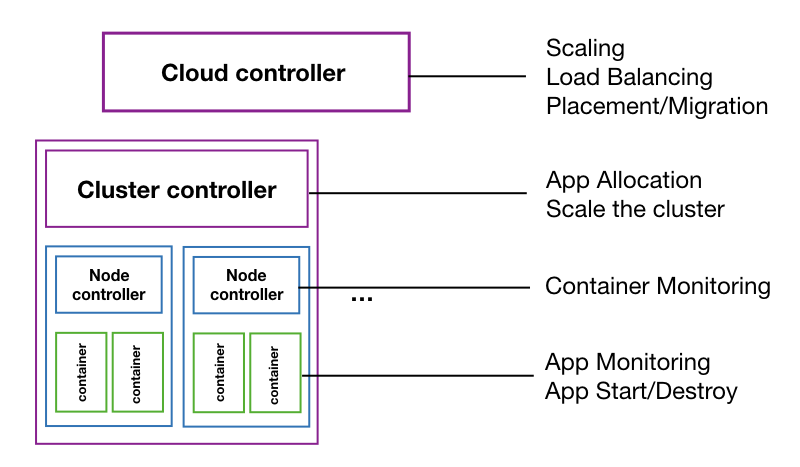
\includegraphics[width=0.7\textwidth]{pics/container-arch.png}
% 	\caption{A resource management architecture of container-based clouds and the functionalities of each layer.}
% 	\label{fig:container_architecture}
% \end{figure}

% \bx{Container-based server consolidation has to consider two levels of optimization on three variables - the placement of containers on VMs, the types of VMs, and the placement of VMs.} The detailed discussion is in Section \ref{related_work}.

\subsubsection{Comparison between Container-based and VM-based virtualization} 
\label{sec:comparison_container_vm}
\bx{This section summarizes three disadvantages of VM-based virtualization in terms of energy efficiency and shows how container-based can overcome these disadvantages based on several research~\cite{Felter:2015ki, Xavier:2013fy, Dua:2014bw}.}  


Some main disadvantages in VM-based virtualization are listed as follows:
\begin{itemize}
	\item Resource over-provisioning \\
	\bx{Cloud users tend to reserve more resources for ensuring the Quality of Service at peak hours \cite{Chaisiri:2012cva} which leads to low resource utilization.} Cloud users do not completely rely on auto-scaling because auto-scaling is more expensive than reservation. However, the peak hours only account for a short period, therefore, for most of the time, resources are wasted.

	\item Unbalanced usage of resources \\
	\bx{Specific applications consume unbalanced resources which leads to a vast amount of resource wastage \cite{Tomas:2013iv}. }For example, computation intensive tasks consume much more CPU than RAM; a fixed type of VM provides much more RAM than it needs. Because the tasks use too much CPU, they prevent other tasks from co-allocating. This also causes wastage.

	\item Heavy overhead of VM hypervisors and redundant operating systems (OSs) \\
	\bx{Heavy overhead of  hypervisors and redundant OSs running in the PM also causes huge resource wastage.} Traditional VM provides a complete independent environment for deploying software which includes its own OS and libraries. However, as most applications only require a general OS such as Windows or Linux, multiple duplicate OSs running in the system is a waste of resource.
\end{itemize}


Some key characteristics of containers can help overcome the above disadvantages of VMs.

The following two characteristics can overcome the heavy overhead of VM hypervisors and reduce the redundant OSs.
\begin{itemize}
	\item Container-based virtualization has lightweight management which generates much less overhead than a VM hypervisor. 
	\item Container-based virtualization shares OSs which reduces the overhead of multiple OSs while VMs have to run separate OSs.

	% \item Container-based virtualization has a near-native performance of CPU, memory, disk and network while VM has a poor I/O performance \cite{Shafer:2010vh}: up to 50\% reduction of bandwidth (e.g hard disk and network). This defect also has a negative effect on the migration performance, since a VM-image is ranging from hundreds of MB to several GBs. 
	\item Container-based virtualization naturally supports vertical scaling while VM-based virtualization does not. Vertical scaling means a container can dynamically adjust its resources under the host's resource constraint. This feature offers a fine granularity management of resources. 

\end{itemize}

	Vertical scaling can overcome the resource over-provisioning by dynamically adjusting the size of containers. Furthermore, the size of container reflects the requirement of the application. We can achieve a balanced usage of resources by using appropriate placement algorithm.

% \bx{These advantages together with fine granularity resource management of container, can be used to \textbf{improve the energy efficiency} by overcoming three main defects in traditional VM-based cloud data centers.}


\bx{In summary, container-based virtualization has the potential to further improve the energy efficiency than VM-based virtualization.} No matter which virtualization technology is used, cloud often deals with three placement decision scenarios. 
% \tran{Next section will introduce the major strategy that is used to reduce the energy consumption in cloud data centers.}




\subsection{Placement Decision Scenarios}
\label{sec:scenarios}

\bx{Three placement decision scenarios \cite{Svard:2015ic, Mishra:2012kx}: initial placement of application, periodic placement of application, and dynamic placement of application (see Figure \ref{fig:management}).}

\begin{figure}
	\centering
	\begin{subfigure}[b]{0.9\textwidth}
		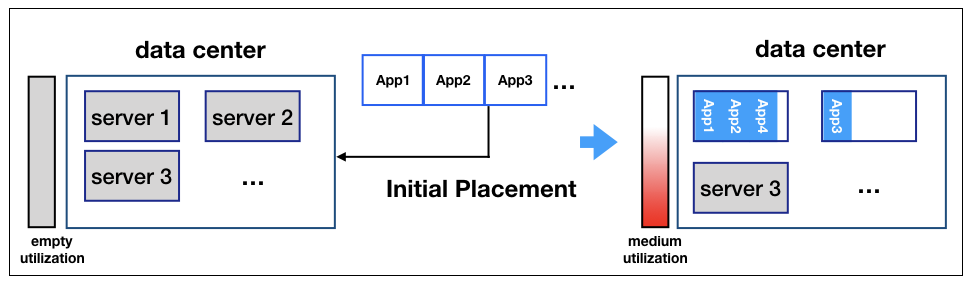
\includegraphics[width=\textwidth]{pics/initial_placement.png}
		\caption{Initial placement of application}
	\end{subfigure}
	\begin{subfigure}[b]{0.9\textwidth}
		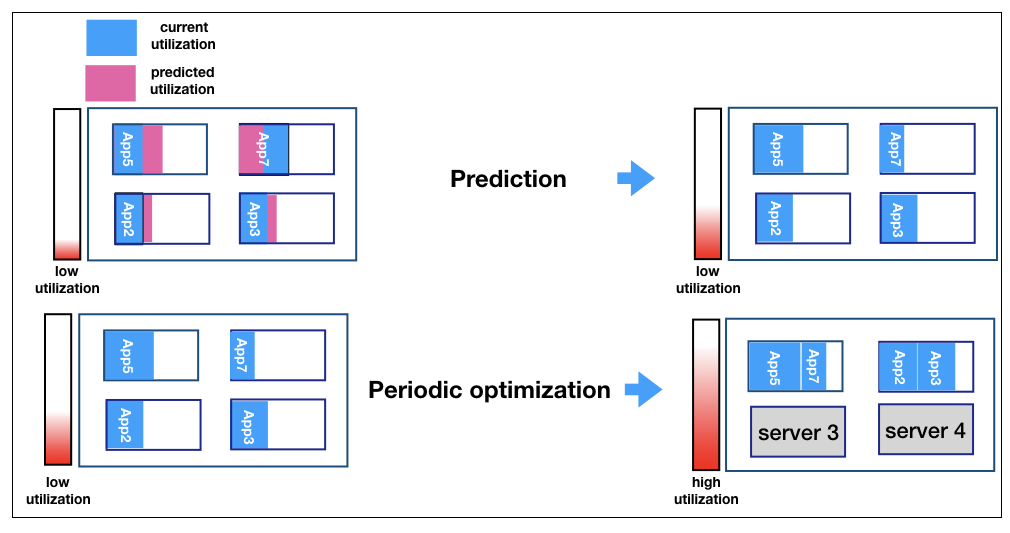
\includegraphics[width=\textwidth]{pics/periodic_optimization.png}
	\caption{Periodic placement of application}
	\end{subfigure}
	\begin{subfigure}[b]{0.9\textwidth}
		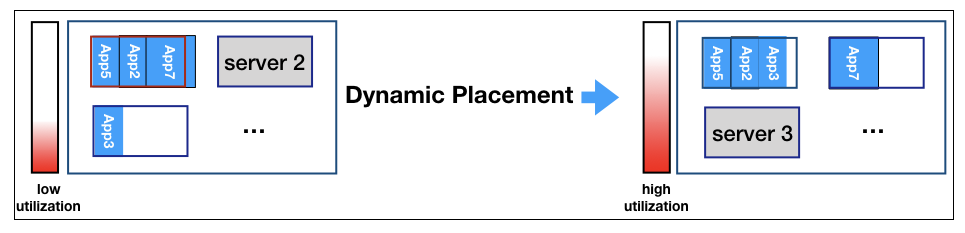
\includegraphics[width=\textwidth]{pics/dynamic_placement.png}
	\caption{Dynamic placement of application}
	\end{subfigure}
	\caption{Three scenarios of placement decision}
	\label{fig:management}
\end{figure}

% Data center constantly receives new requests for applications initialization. Once the new applications have been allocated, the utilization begins to drop. This is because, initially, applications are compactly allocated on PMs. As old applications instance are released because of canceling, the compact structure become loose. Dynamic resource management is a process which can slow the utilization from decreasing. It consolidates by re-allocating one application at a time. Finally, global consolidation is conducted periodically to dramatically improve the resource utilization.
\paragraph{Initial placement of application} is applied when new applications arrived. The task is to place applications into a set of PMs \cite{Mishra:2012kx} so that PMs satisfy all applications' resource demands and minimize the energy consumption.

% In VM-based cloud, this problem is often modeled as a single level bin-packing problem \cite{CoffmanJr:1996ui}. In container-based clouds, an extra level of placement - containers to VMs - need to be considered. Two levels of placement: Container-VM, VM-PM, interact with each other. The problem is modeled as a bilevel optimization problem \cite{Mathieu:2011dw} where each level is a bin-packing problem. Previous approaches are based on VM-based cloud, therefore, they cannot be used in the bilevel problem.


\paragraph{Periodic placement of application} is applied periodically to adjust the current placement of applications. The task is to re-place the current applications so that resource management minimizes the energy consumption and minimizes the cost of migration.

% Similar as initial placement of application, container-based periodic placement of application is also a bilevel optimization problem. In addition, previous works only consider applications' workload as static, therefore, it incurs more migration afterwards. In practice, the types of workload should be considered into the decision process.

	% In this problem, time is discrete and it can be split into basic time frames, for example: ten seconds. A periodical operation is conducted in every $N$ time frames.
	% A cloud data center has a highly dynamic environment with continuous arriving and releasing of applications. Releasing applications cause hollow in PMs; new arrivals cannot change the structure of current allocation. Therefore, after the initial allocation, the overall energy efficiency is likely to drop along with time elapsing. 

	% In prediction, an optimization system takes  the current applications' utilization records as the input. Make a prediction of their utilization in the next period of time. 
	% In Global consolidation, based on the predict utilization and the current allocation - including a list of applications/VMs and a list of PMs, the system adjusts the allocation so that the global resource utilization is improved.

	% In comparison with initialization, instead of new arrivals, the global consolidation considers the previous allocation. Another major difference is that global consolidation needs to minimize the differences of allocation before and after the optimization. This is because the adjustment of allocation relies on a technique called live migration \cite{Clark:2005ud}, and it is a very expensive operation because it occupies the resources in both the host and the target. Therefore, global optimization must be considered as a time-dependent activity which makes the optimization even difficult.

	% In comparison with dynamic consolidation, global consolidation takes a set of VMs as input instead of one. Therefore, it is time consuming and often treated as a static problem.

\paragraph{Dynamic placement of application} is applied in two scenarios \cite{Mishra:2012kx}: Overloading and underloading. Overloading is a scenario where the total demands of applications in a PM are higher than the PM's resources. Therefore, the PM causes a degradation in one or more applications' performance. Underloading is a scenario where the PM is running in low utilization. In both scenarios, resource management moves the applications from one PM to another PMs in an on-line fashion~\cite{Borodin:2cY4439E}.



	% No matter which scenario it is, a dynamic resource management always involves three steps . 
	% \begin{itemize}
	% 	\item \emph{When to migrate?} refers to determine the time point that a PM is overloaded or underloaded. It is often decide by a threshold of utilization.
	% 	\item \emph{Which application to migrate?} refers to determine which application need to be migrated so that it optimize the global energy consumption.
	% 	\item \emph{Where to migrate?} refers to determine which host that an application is migrated to. This step is called dynamic placement of application which is directly related to the consolidation, therefore, it is decisive in improving energy-efficiency. 
	% \end{itemize}

	% Among three operations, dynamic placement of application is a dynamic and on-line problem.
	% The term ``dynamic'' means the request comes at an arbitrary time point. An on-line problem is a problem which has on-line input and requires on-line output . It is applied when a control system does not have the complete knowledge of future events.

% 	There are two difficulties in this operation, firstly, dynamic placement of application requires a fast decision while the search space is very large (e.g hundreds of thousands of PMs). Secondly, migrate one application at a time is hard to reach a global optimized state.

% \end{enumerate}

% Finally, a consolidation plan includes four major items:
% 			\begin{enumerate}
% 				\item A list of existing PMs after consolidation
% 				\item A list of new virtual machines created after consolidation
% 				\item A list of old PMs to be turned off after consolidation
% 				\item The exact placement of applications and services
% 			\end{enumerate}


% \subsection{VM-based Static Consolidation Techniques}
% \label{sec:static}

% In summary, resource management allocates resources to Cloud users to run their applications. From technology's perspective, the recent container-based clouds has three advantages than traditional VM-based cloud in terms of energy efficiency. From the procedure of resource management, cloud often encounters three placement decision scenarios. 

Next section will discuss server consolidation strategies in three scenarios based on the two types of virtualization: VM and container.


\section{Related Work}
\label{sec:related_work}
% In this section, we summarize the related works in the terms of three resource management processes: initial placement of application, Periodic placement and dynamic consolidation, corresponding to our proposed objectives. In each sub section, we analyze the container-based and VM-based approaches, discuss their models and methodologies. 
Related work discusses the server consolidation strategy and the studies of consolidation strategies on three placement decision scenarios: initial placement, periodic placement, and dynamic placement. 

\subsection{Server consolidation strategy}
\label{consolidation}

\begin{figure}
	\centering
	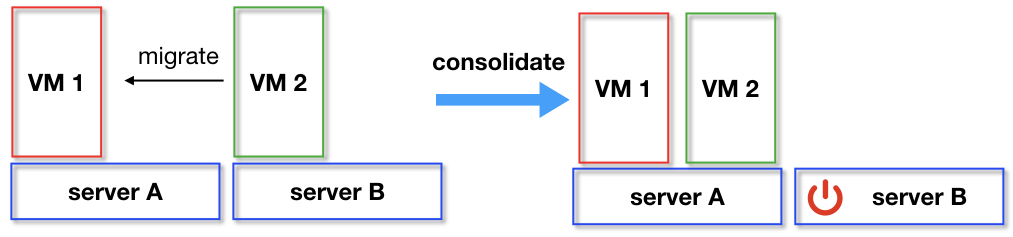
\includegraphics[width=0.7\textwidth]{pics/consolidate.png}
	\caption{A Server Consolidation example: Initially, each PM runs an application wrapped with a VM in a low resource utilization state. After the consolidation, both VMs are running on PM A, so that PM B is turned off to save energy \cite{Barroso:2007jt}.}
	\label{fig:consolidation}
\end{figure}


\bx{Server consolidation is a resource management strategy that aims to improve the utilization of PMs and reduce the energy consumption.} We use VM-based virtualization as an example: a general step of server consolidation is shown in Figure \ref{fig:consolidation}, a number of VMs is migrated to fewer number of PMs. Resource management applies Server consolidation to solve 
the low utilization of PMs called PM sprawl~\cite{Khanna:2006vq}.

% \subsubsubsection{Model}
\begin{figure}
	\centering
	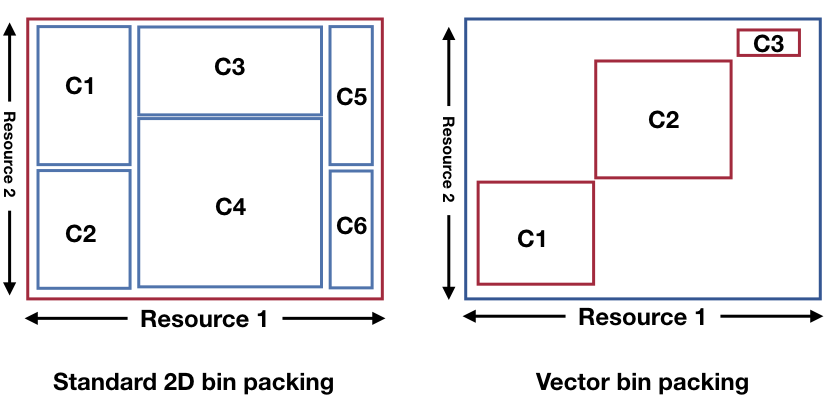
\includegraphics[width=0.6\textwidth]{pics/bin_packing_problem.png}
	\caption{A comparison between standard bin packing and vector bin packing}
	\label{fig:bin_packing_problem}
\end{figure}

\subsubsection{Types of Server consolidation}

% Three major benefits of virtualization make it be the first choice for web-based application consolidation: No reliance on hardware, easy to provision and live migration.

\bx{Server consolidation can be done in two ways: Static and dynamic \cite{Xiao:2015ik, Verma:2009wi} based on different scenarios.} Initial placement and periodic placement involve large number of variables, therefore, they are very time-consuming job and often conducted in an off-line fashion. Dynamic placement requires a fast decision-making to place one application to PMs. Thus, resource management uses a dynamic server consolidation strategy to handle the scenario. 


% Several one dimensional bin packing algorithms have been generalized to vector bin packing such as generalized First Fit and Best Fit. In studies \cite{}, they suggest that an algorithm should keep the bins as ``balanced'' as possible, so that bins have better potential to accommodate more items. 

% \subsubsubsection{Server consolidation technologies}

% \textcolor[Maroon]{Why Server consolidation?}
% Physical server sprawl not only wastes valuable computing resources but leads to a waste of energy, as Hameed et al \cite{Hameed:2016cma} addressed, even at a low level of 10\% of CPU utilization, PMs still consume more than 50\% of its peak time. 
% In addition, Han et al \cite{Han:2017jz} state that average resource utilization of PMs  is usually between 10\% to 50\%
% of its capacity. Server consolidation is often used to solve the disproportionate between utilization and energy consumption \cite{Barroso:2007jt}.

% \textcolor[Maroon]{How to do server consolidation?}




% \textcolor{Maroon}{To understand the relationship among providers and users, we first illustrate the stakeholders of Cloud computing.} (see Figure \ref{fig:stakeholders}): Cloud providers, Cloud users (applications providers), and End (application) users \cite{Jennings:2015ht}. Cloud providers build data centers, provide maintenance and resource management on hardware infrastructures such as servers. Cloud users develop and deploy applications on Cloud infrastructures. End users consumes applications developed by Cloud users and hosted by Cloud providers. 

% Cloud computing has made one critical change in software industry, it separates the role of traditional service provider into service provider and infrastructure provider. As Wei \cite{Wei:2010fn} states, ``one provides the computing of services, and the other provides the services of computing''. Therefore, this separation add one more layer between service provider and users, as: Cloud providers, Cloud users (service providers), and End users \cite{Jennings:2015ht} . 


% The detailed goal and objectives of stakeholders are described below. 


% \begin{itemize}
% 	\item \emph{Cloud providers}' goal is to increase the profit by boosting the income and reducing the expense. Their income comes from Cloud users' rental of servers or \emph{Physical Machines (PMs)} in terms of resource quality (e.g  3.5GHz dual-core CPU), quantity (e.g 3 PMs), and time (e.g 1 year). Therefore, Cloud providers objective is to maximize utilization of computing resources. A high utilization brings two benefits, firstly, it increases income by accommodating more applications in limited resources. Secondly, it cuts the expense of energy consumption by packing applications in a minimum number of PMs so that idle PMs can be turned off. 	
% 	\item \emph{Cloud users}' goal is also to increase the profit mainly through two objectives, attracting more End users and reduce the expense of resources. The first objective can be achieved by improving the quality of service as well as lower the fee for End users. Either way depends not only on the software entities but also the quality of service (QoS) offered by Cloud provider. The second objective can be achieved by a good estimation of the reserved resources, so that they do not rent insufficient  or too much resources which cause performance degradation or wastage.
% 	\item \emph{End Users}' goal is to obtain a satisfactory service. It is achieved by signing a Service Level Agreement (SLA) with Cloud users which constrains the performance of the services.
% \end{itemize}

% \textcolor{Maroon}{Cloud service models describe the responsibilities and obligations of stakeholders.}
% Cloud computing has three traditional service models \cite{Mell:2011jj}: Infrastructure as a Service (IaaS), Platform as a Service (PaaS) and Software as a Service (SaaS). The relationship among three service models is showed in Figure \ref{fig:architecture}. 
% Service models of Cloud computing are critical in solving energy consumption problem because their distinct ways of managing resources have sever effect on the problem. These distinct ways of resource management mainly result from the responsibilities among stakeholders. 

% \begin{figure}
% 	\centering
% 	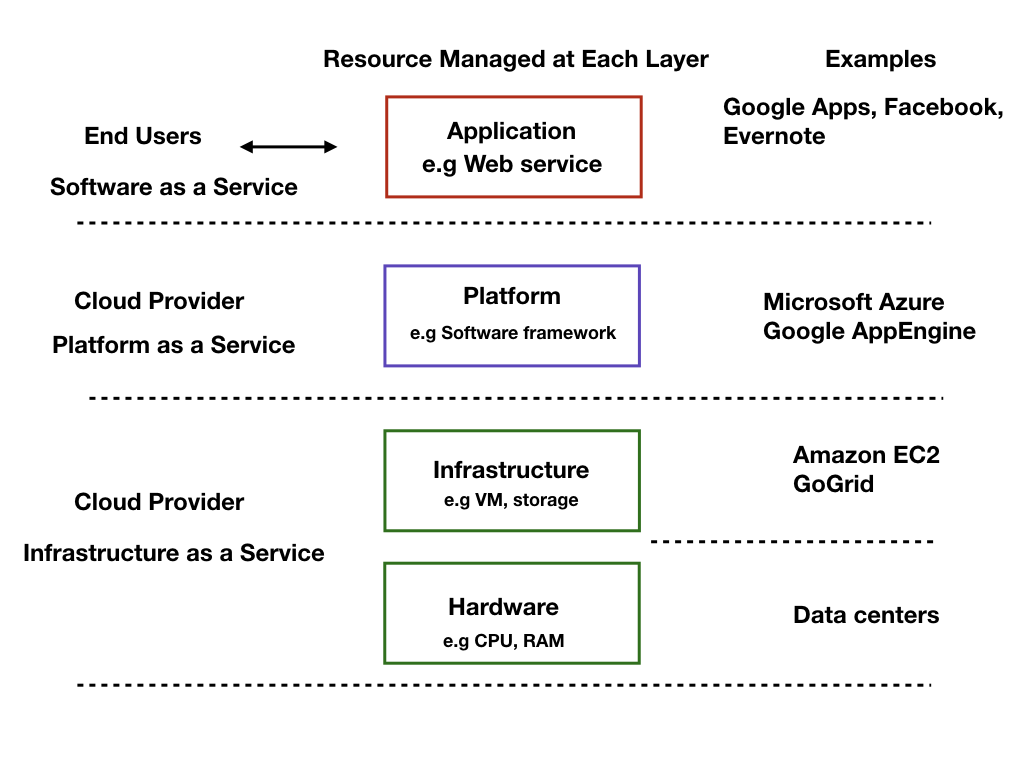
\includegraphics[width=0.9\textwidth]{pics/architecture.png}
% 	\caption{Cloud computing architecture \cite{Zhang:2010vo}. 
% 	IaaS provides the fundamental resources such as CPU cores, RAM. The resources are usually wrapped with various types of virtual machine. PaaS provides a software platform sitting on top of IaaS for Cloud users to develop applications. SaaS describes the relationship between applications and End Users.}
% 	\label{fig:architecture}
% \end{figure} 

% \begin{itemize}
% 	\item IaaS, a Cloud provider hosts hardwares such as PMs and cooling infrastructure on behalf of Cloud users. Computational resources are often encapsulated in virtualized computing units called virtual machines (VMs). Cloud providers establish a number of types of VM for simplifying the management. The `type' means a VM contains a certain quantity of resources such as 2-cores and 1 GB RAM.  \emph{Traditional} IaaS and PaaS use VM as the fundamental unit of resources.

% 	A typical procedure of an application deployment includes several steps.
% 	Initially, the Cloud user estimates the resources that their applications might consume and selects a type of VM which can satisfy the requirement. After the Cloud user has made the decision, he/she sends requests to Cloud providers for a number of VMs. Finally, Cloud providers received the request, provisioned and allocated these VMs to PMs. 

% 	% From the resource management perspective, the constraint in allocation of VMs is that the aggregated VMs' resources in a PM cannot exceed the capacity of the PM. After these VMs have been allocated, their types cannot be changed. During the life cycle of an application, Cloud providers can dynamically adjust the locations of VMs, provision new VMs (same type) for the replicas of an application, as well as turning on/off PMs.

% 	% After receiving the requests, Cloud providers choose a set of PMs which contains sufficient resources, provision the required VMs in them. Then, the VMs are assigned to the Cloud users. Cloud providers manage the VMs by monitoring the resource utilization of VMs and PMs. If a VM has run out of resources, an auto-scaling strategy is used to provision new VMs to Cloud users. Finally, Cloud providers optimize the locations of VMs so that the energy consumption of data center is minimized.


%  	\item PaaS, a Cloud provider offers a platform which allows Cloud users to develop, test and deploy their applications on it.

%  	From resource management perspective, PaaS is sitting above the IaaS which means the underlying resource is still based on IaaS VM types. Different from IaaS, PaaS takes the responsibility of selecting VMs and allows Cloud users to focus on software development. 

 	% A typical procedure of a Cloud user deploying their applications in an PaaS cloud includes several steps.
 	% In the first step, Cloud users need to provide the initial estimation of the quantity of resources instead of types of VM. Then, Cloud providers determine the types of VM for applications according to the estimated resources.  After this step, resource management system conducts the provisioning and allocating as the same steps in IaaS. During the life cycle of applications, similar to IaaS, Cloud providers can also adjust the location of VMs, add new VMs, and control the status of PMs. Different from IaaS, Cloud providers can change the type of VM for an application as long as the application's performance can be guaranteed.

 	% The system monitors the utilization of a number of PM and VM and through adjustment of their location to optimize the energy consumption of the data center. The input is a list of VMs (e.g CPU cores and RAMs) and a list of PMs. The task is to put the VMs into these PMs so that the VMs only use a minimum number of PMs. The sizes of VMs and PMs are fixed. A system can only adjust which VM is allocated to which PM. A general constraint is the sum of resources of the VMs inside a PM cannot exceed the capacity of the PM.

%  	\item SaaS, Cloud users develop applications and deploy them on Cloud so that End users can access them via the Internet. Although this service model does not directly related to the resource management, it provides the fundamental reasons for resource management and optimization: applications receive fluctuated requests from End users. Because of the dynamic nature of workloads, the underlying resources must also be dynamic adjusted to meet the requirement.
% \end{itemize}
 
% \subsection{Drawbacks of Traditional Service Models}

% There are three characteristics in IaaS which naturally lead to a low resource utilization.
% \begin{itemize}
% 	\item Resource over-provisioning \\
% 	As previous mentioned, VMs are either selected by Cloud users or automatically selected by software platforms. In either case, it requires an estimation of required resources. However, The accurate estimation is almost impossible because of unpredictable workloads; A simple way is to reserve more resources for ensuring the QoS at peak hours \cite{Chaisiri:2012cva}, rather than completely rely on auto-scaling, simply because auto-scaling is more expensive than reservation. However, the peak hours only account for a short period, therefore, in most of time, resources are wasted. In IaaS, the types of VM are a part of the contract, Cloud providers cannot simply change the type of VMs after provisioning.

% 	\item Unbalanced usage of resources \\
% 	Specific applications consume unbalanced resources which leads to vast amount of resource wastage \cite{Tomas:2013iv}. For example, computation intensive tasks consume much more CPU than RAM; a fixed type of VM provides much more RAM than it needs. Because the tasks use too much CPU, they prevent other tasks from co-allocating. This also causes wastage.

% 	\item Heavy overhead of VM hypervisors and redundant operating systems (OSs) \\
% 	% Redundant operating systems (OSs) cause vast resource wastage. \\ 
% 	In VM-based resource allocation, heavy overhead is caused by
% 	the hypervisor of VMs and the separated operating systems running in the PM. A hypervisor manages and monitors the VMs running on a PM. The overhead of a hypervisor is heavier with the increasing numbers of VM. Redundant operating system is another reason for overhead, as normal applications do not need specific operating systems; Commonly used OSs - such as Linux-based: RedHat, or Windows server versions - are well enough for their needs. Therefore, running applications in separated operating system simultaneously is unnecessary.
% \end{itemize}


% For traditional PaaS, Cloud providers can adjust the VMs' location and the type of VMs. Therefore, it overcomes the first drawback of IaaS. Because of PaaS is built upon IaaS, the one-on-one relationship between application and VM still exist. PaaS can only select the most suitable type instead of changing their sizes. Therefore, the unbalanced resource problem cannot be solved. In addition, PaaS brings a restriction for the applications deployed on it. PaaS build a software middle-ware to allow Cloud users' development. The middle-ware requires the deployed applications to be compatible with the environment, for example, Google App engine only allows certain programming languages and libraries. Therefore, the generality of PaaS is limited. It is urgent to provide a environment which supports automatic resource management as well as an editable programming environment.


% \subsection{Container as a Service}
% \textcolor{Maroon}{Container as a Service (CaaS) \cite{Piraghaj:2017vi} is a new service model which is usually considered as a combination of IaaS and PaaS.} CaaS uses containers and VM as its fundamental resource allocation unit as shown in Figure \ref{fig:comparison} on the right hand side. 


% \textcolor{Maroon}{CaaS has advantages of both IaaS and PaaS but without their disadvantages.} On one hand - similar to PaaS - CaaS allows Cloud providers to manage resource in a fine granularity with containers, therefore, it may lead to high utilization of resources. On the other hand - similar to IaaS - CaaS allows customers to customize their software environment without being constrained by platforms. Therefore, it has more flexibility than PaaS.



% Later, multiple ways of dynamic migration (e.g pre-copy \cite{Clark:2005ud} and post-copy \cite{Hines:2009fv}) of VM were invented, which compresses and transfers a VM from one PM to another. This technique allows resource management in real time which inspires the strategy of server consolidation. 

	
% On the other hand, the disadvantages of containers are categorized in two aspects. Currently, containers have rather poor performance in isolation for memory, disk, and network. Security is immature in containers \cite{Bernstein:2014ur}, therefore, high security required applications are not recommended to be deployed in such systems. 


% \subsection{Evolutionary Computation}
% Evolutionary Computation is a subfield of Artificial Intelligence. It is very well-known for its effective global search ability. These algorithms are 
% inspired by biological mechanisms of evolution, social interactions and swarm intelligence. 
% There are several distinguished characteristics of EC algorithms such
% as the use of a population-based search and the ability of avoiding local optima. 
% A common process of EC algorithms is as follows. Initially, the population are randomly generated in the search space. During the evolution process, the population
% explores according to the evaluation of a or multiple predefined fitness functions. At the end of the evolution, the individual with the best fitness value is selected as the output.

% The origins of evolutionary computation can be traced back to 1950s \cite{Back:1997gb}. Since 1970s, the output of EC research has grown exponentially. 
% The majority of current implementations of EC algorithms descend from three major approaches: \emph{genetic algorithms}, \emph{particle swarm optimization}
% and \emph{genetic programming}.

% \subsubsection{Genetic Algorithm}
% GA \cite{Holland:1962fy} was introduced by Holland. Since then, a large number of applications \cite{DeJong:1992vk, DeJong:1992ws} have applied GA  as their search mechanism. In a GA, a population of chromosomes which represents the solutions of the problem are often represented as a fixed length string. Each entry or bit can be continuous, discrete or even alphabets depending on the problem.  The evolution often starts from randomly generated population followed by an iterative process called generation.  In each generation, the fitness value of chromosomes is evaluated according to a defined fitness function.  Then, genetic operators such as mutation, crossover are applied on the solutions so that they are modified. As a search mechanism, these operators move solutions to explore the search space. New generation of solutions are then evaluated by the fitness function.  This evolutionary procedure ends with a predefined a generation number or a satisfactory level of fitness has been reached.

% \begin{figure}
% 	\centering
% 	\begin{subfigure}[b]{0.44\textwidth}
% 		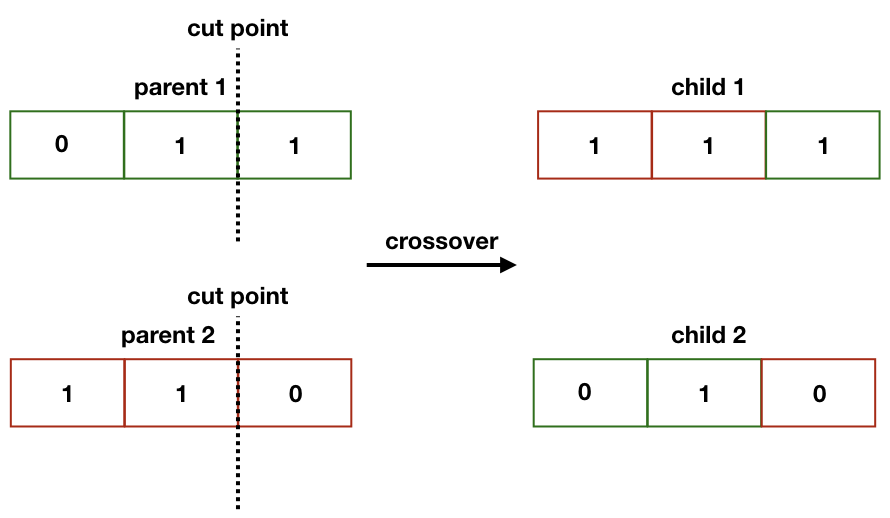
\includegraphics[width=\textwidth]{pics/crossover.png}
% 	\caption{Crossover}
% 	\end{subfigure}
% 	\begin{subfigure}[b]{0.44\textwidth}
% 		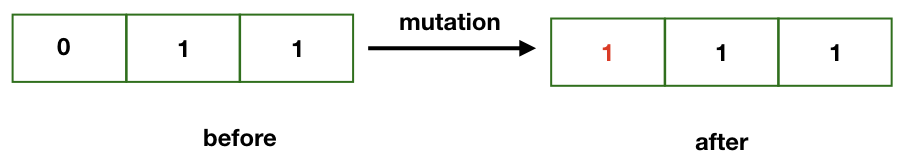
\includegraphics[width=\textwidth]{pics/mutation.png}
% 	\caption{Mutation}
% 	\end{subfigure}
% 	\label{fig:operators}
% \end{figure}
% % Evolutionary programming, introduced by Fogel \cite{Fogel:1962wv}, was originally designed to generate artificial intelligence. 
% % Evolutionary strategies as developed by Rechenberg \cite{Rechenberg:a_aZDNtZ} and Schwefel \cite{Schwefel:Nd2pzTwG}, were initially designed with the goal of solving difficult discrete
% % and continuous, mainly experimental, parameter optimization problems \cite{Klockgether:1970tw}. 

% \subsubsection{Particle Swarm Optimization}
% Kennedy and Eberhart proposed PSO in 1995 \cite{Eberhart:1995tj}. It is a meta-heuristic algorithm inspired by the social behavior of birds. In PSO, each individual - a particle - searches the solution space. The underlying phenomenon of PSO is to use the collective knowledge to find the optimal solution.

% At the initial state, each particle has a random initial position in the search space which is represented by a vector $\vec{x}_i = (x_{i1}, x_{i2}, \dots, x_{iD})$, where \emph{D} is the dimension of the search space. A particle has a velocity as $\vec{v}_i = (v_{i1}, v_{i2}, \dots, v_{iD})$. The velocity is limited by a threshold $v_{\max}$ so that for any $i$ and $d$, $v_{id} \in [-v_{\max}, v_{\max}]$. During the search process, each particle maintains a record of its best position so far, called the \emph{personal best} ($pbest$). The best positions among all the personal best positions of its neighbors is the \emph{global best} ($gbest$). The position and velocity of each particle are updated according to the following equations:
% \begin{equation}
% \label{eq:updatePosition}
% x^{t+1}_{id} = x^{t}_{id} + v^{t+1}_{id},
% \end{equation}

% \begin{equation}
% \label{eq:updateVelocity}
% v^{t+1}_{id} = w \cdot v^{t}_{id} + c_1 \cdot r_{1i} \cdot (p_{id} - x^t_{id}) + c_2 \cdot r_{2i} \cdot (p_{pg} - x^i_{id}).
% \end{equation}

% Here, $t$ is the index of iteration. $d$ is the index of dimension. The inertia weight $w$ is used to balance the local search and global search abilities. The parameters $c_1$ and $c_2$ are the acceleration constants. $r_{1i}$ and $r_{2i}$ are random constants following the uniform distribution in the interval $[0, 1]$. $p_{id}$ and $p_{gd}$ denote the values of $pbest$ and $gbest$ in the $d^{th}$ dimension of the $i^{th}$ particle.

% PSO was initiated to solve continuous optimization problems - position update function is developed for real numbers. To address discrete problems, Kennedy and Eberhart developed a binary PSO \cite{Kennedy:1997hd}. 

%



% Static initialization, is also frequently referred to initial placement problem \cite{Jennings:2015ht}. Whenever a request for provisioning of applications by one or more Cloud users. The resource management system schedules the applications into a set of PMs. Currently, most state-of-the-art research focus on VM-based placement, in this case, applications are installed in VMs. Therefore, ``application placement'' and ``VM placement'' are used interchangeable in the literature. 

% In energy-aware resource management, the initialization has the objective of minimizing the used PMs. In literature, the static initialization problem is often modeled as the vector bin packing problem. Each application represents an item and PMs represents bins.



\subsection{Initial placement of application}
\label{sec:initial}

This section first discusses server consolidation strategies on container-based virtualization and VM-based virtualization.

% since there are only few research study the  container-based placement and none of them considers it as a bilevel optimization problem, specifically, each level of optimization problem is a bin packing problem.  


% We will first review a number of approaches solving the problem with traditional bin packing approaches. Then, a number of advanced approaches will be examined. We mainly study the following five aspects: resource model, power model, wastage model, objective, and algorithm.
% In energy-aware resource management, the initialization has the objective of minimizing the used PMs. In literature, the static initialization problem is often modeled as the vector bin packing problem. Each application represents an item and PMs represents bins.

\subsubsection{Container-based initial placement of application}
\label{container-based-placement}
This section will discuss existing approaches for Container-based initial placement. Then, we will describe a potentially way of modeling energy consumption in container-based virtualization: a bilevel model. Last, we will illustrate a number of algorithms to solve bilevel optimization problems. 


\paragraph{Existing approaches}

\bx{We discuss two research works on container-based virtualization: Piraghaj et al \cite{Piraghaj:2016bw} and Mann \cite{Mann:2016hx} on their similarities and differences.} Two papers both consider two resources: CPU and memory. The constraints on these resources are the containers cannot exceed the resources in their located VMs. Both research do not include the balance of CPUs and memories. In contrast, in most VM-based approaches (discussed in next section) consider the balance.

\bx{The first difference between two papers is that Mann considers the overheads of VM.} Mann models the overhead as a constant value of CPU utilization but he mentioned more sophisticated models can be more realistic. On the other hand, Piraghaj et al \cite{Piraghaj:2016bw} adopt a widely used VM-based linear energy model~\cite{Xavier:2017jl} and does not consider the overheads of VM. 

The second difference is their resource management architectures. The architecture in Piraghaj's research allows adjusting 
the size of VMs when allocating new applications, while in Mann's work, containers runs on top of a traditional IaaS where containers must choose to allocate to a type of VM. 

The third difference is their distinct ways to achieve initial placement based on their different architectures of resource management. Piraghaj considers the initial placement a two-steps procedure: containers to VMs and VMs to PM. Because their resource management allows cloud providers to customize the size of VMs, in the first step, they must first determine the size of VM. Piraghaj performs clustering technique on historical workload data from Google Cluster Data. In this way, Piraghaj suggests that the applications with similar workload pattern can be categorized into the same group. In the placement step, Piraghaj designs a simple heuristic: in both VM and PM levels, they apply First Fit algorithm. Then, the containers are allocated to certain size of VMs. Piraghaj claims that their main contribution is not the placement strategy but an architecture for container-based resource management. On the other hand, Mann realizes this two-levels of placement are interact with each other, therefore, container-VM and VM-PM must be considered collaboratively. Specifically, the initial placement of application becomes three parts: 

\begin{itemize}
	\item VM size selection for containers
	\item Container placement
	\item VM placement
\end{itemize}

% However, another concern is ``why not placement as many containers as possible in a single VM which minimizes the overhead of hypervisor''. The paper gives an answer of ``Too big VMs limit the consolidation possibilities''. 
In order to prove interaction of two-levels of placement, Mann fixed a VM placement algorithm and tested a series of VM selection algorithms such as simple selection \cite{Ganesan:2012eb},  Multiple selection, Maxsize, Consolidation-friendly. Mann discovers that the final energy consumption varies with the selection algorithms. Mann claims that the performance is better when VM selection has more knowledge of the PMs' capacity. However, Mann's study only focuses on the partial placement with fixed VM placement algorithm. The answer of ``How these two-levels of placement interact ?'' is still undiscovered.


\bx{We have two reasons to propose a distinct approach from Piraghaj \cite{Piraghaj:2016bw} to solve the container-based placement problem.} First, Piraghaj's architecture can create arbitrary size of VM when requests arrive. In contrast, our assumption is that the container-based architecture is based on traditional IaaS, where fixed-size VMs provide the fundamental resources. Second, from the perspective of energy efficiency, the allocation of container and VM interact with each other. That is, the minimum number of VMs does not necessary lead to the minimum number of PMs, because the type of VMs also affect the results. Therefore, Piraghaj's approach cannot guarantee a near optimal energy consumption. This inspires us to simultaneously allocate containers and VMs. 

% In addition, both approaches do not consider the OS requirement of containers as a constraint. We argue that this is another critical reason for deploying containers into different VMs.

In order to solve the problem, we believe a promising way is to model the energy consumption in container-based virtualization as a bilevel optimization~\cite{Colson:2007bu} (described in the next section). Bilevel optimization represents the interaction so that a bilevel optimization algorithm can solve the energy consumption problem. Next section will introduce the basic structure of a bilevel model or a bilevel optimization.

% The main challenge is that solving a bilevel optimization is NP-hard~\cite{Sinha:2013tn}. Traditional approaches such as Branch-and-bound \cite{Bard:1982gsa} can only be applied in very small problems. Evolutionary algorithms, on the other hand, become popular approaches in bilevel optimization \cite{Wang:2005fa, Sinha:2013tn}. 



\paragraph{Bilevel optimization}
\label{bilevel}

% \bx{The joint allocation of container and VM can be modeled as a bilevel optimization.}
A bilevel optimization \cite{Colson:2007bu} is a kind of optimization where one problem is embedded within another.
 % The outer optimization is referred to as the \emph{upper-level} problem, while the inner optimization is referred to as the \emph{lower-level} problem. 
The general formulation of a bilevel optimization problem can be defined as: 

\begin{subequations}
\label{eq:bilevel}
	\begin{align}
	min_{x \in X, y} 	\quad F(x, y) \\
	s.t 			\quad G(x, y) \leq 0, \\
	min_y			\quad f(x, y) \\
	s.t 			\quad g(x, y)
	\end{align}
\end{subequations}

The lower-level problem is the function $f(x, y)$, where the decision variable is $y \in \mathbb{R}^{n_2}$. The upper-level problem is the function $F\{x, y\}$ where the decision variable is $x \in \mathbb{R}^{n_1}$.
The function $F : \mathbb{R}^{n_1} \times  \mathbb{R}^{n_2} \to \mathbb{R}$ and $f : \mathbb{R}^{n_1} \times  \mathbb{R}^{n_2} \to \mathbb{R}$ are the \emph{upper-level} and \emph{lower-level objective functions} respectively. The function $G : \mathbb{R}^{n_1} \times  \mathbb{R}^{n_2} \to \mathbb{R}^{m_1}$ and $g : \mathbb{R}^{n_1} \times  \mathbb{R}^{n_2} \to \mathbb{R}^{m_2}$ are called the \emph{upper-level} and \emph{lower-level constraints} respectively. 

Bilevel optimization problem has a hierarchical structure. This structure may introduce difficulties such as non-convexity and disconnectedness even for simple cases such as bilevel linear programming problems is strongly NP-hard \cite{Sinha:2013tn}. 

In practice, there are a number of problems that are bilevel in nature. For example, transportation related: work design, optimal pricing \cite{Brotcorne:2001je, Constantin:1995hu}, management: network facility location \cite{Sun:2008gq},  and engineering related: optimal design \cite{KirjnerNeto:1998ef}. 




\paragraph{Existing approaches for Bilevel optimization}

A number of studies have been conducted on bilevel optimization \cite{Colson:2007bu,Dempe:2006jc}. Approximation algorithms such as Karush-kuhn-Tucker approach \cite{Bianco:2009ej, Herskovits:2000be}, branch-and-bound \cite{Bard:1982gsa} are often applied to solve bilevel problems. Most of these approaches are not applicable when the problem size increases.
% Heuristics such as Evolutionary methods have been applied for solving bilevel optimization problem with higher level of complexity \cite{Yin:2000bt,Wang:2008kb}. 

Evolutionary methods have been applied to bilevel optimization problem since 90s. Mathieu et al \cite{Mathieu:2011dw} proposed an genetic algorithm (GA) based approach. It uses a nested strategy - the lower level is optimized with a linear programming method and the upper level apply a GA.

Oduguwa and Roy \cite{Oduguwa:2002kr} proposed a co-evolutionary approach for bilevel problems. Two population are co-operated to find the optimal solution, where each population handles a sub-problem. 

Wang et al \cite{Wang:2005fa} proposed an evolutionary algorithm based approach with a constraint handling technique.  Their approach is able to handle non-differentiability at the upper level objective function, but not in constraints and lower  level objective function. Later on, Wang proposed an improved version \cite{Wang:2011di} that shows better performance than the previous version.

Particle Swarm Optimization \cite{Li:2006br} was also used in solving bilevel problems.
A recent work is from Sinha et al \cite{Sinha:2013tn}, they propose a bilevel evolutionary algorithm (BLEAQ) works by approximating the optimal solution mapping between the lower level optimal solutions and the upper level variables.  BLEAQ was tested on two sets of test problems and the results were compared with WJL \cite{Wang:2005fa} and WLD \cite{Wang:2011di}. The results show BLEAQ is much faster than previous approaches.
One major drawback of evolutionary algorithms is its high computation cost which limits the problem size from growing bigger.

In conclusion, as the complexity of the problem, practical problems with bilevel nature are often simplified into a single-level optimization problem which can achieve a satisfactory level instead of optimal. Classic algorithms often fail because of the nature of bilevel problem such as non-linearity, discreteness, no-differentiability, non-convexity etc. EC algorithms have been successfully applied on bilevel problems.



% Without this constraint, all containers can be simply allocated to homogeneous VMs which can be solved by traditional VM-based approaches.

% Mesos \cite{Hindman:2011ux} is a platform for sharing commodity clusters between cluster computing frameworks such as Hadoop and MPI. It has a two-level of resource allocation architecture where a master node and several slave node. A master node only decides how many resources to offer to each framework (slave) based on fair sharing policy \cite{Ghodsi:2011vm}. Each slave node belongs to a cluster framework and it makes the decision of which resources to use. Each framework has to define its allocation policy. Mesos focus on sharing resources across multiple frameworks and has a better scalability since it deligates the application placement to decentralized slave nodes. The main problem for Mesos is that it does not consider energy consumption for Cloud providers with user-defined allocation policy.

\subsubsection{VM-based initial placement of application}
\label{initial_placement}
This section first describes a commonly used energy model for VM-based virtualization: Bin packing model. Then, we review a number of traditional approaches for VM-based initial placement . We mainly study the following five aspects: resources, power model, wastage model (balance between resources), objective, and algorithm.

\begin{table}[]
\centering
\caption{A Comparison of different models and approaches}
\label{vm-based-comparison}
\scalebox{0.7}{
\begin{tabular}{@{}lccccc@{}}
\toprule
\multicolumn{1}{c}{Research}                      & Resources        & Algorithm                     & \multicolumn{1}{l}{Power model} & Wastage model                             & \multicolumn{1}{l}{Objective} \\ \midrule
\multicolumn{1}{c}{Xu et al \cite{Xu:2010vh}}   & CPU and RAM      & GGA and Fuzzy multi-objective & Linear                          & balance  resources & three                         \\
\multicolumn{1}{c}{Gao et al \cite{Gao:2013gg}} & CPU and RAM      & Ant Colony Optimization       & Linear                          & balance  resources & Two                           \\
Ferdaus et al \cite{Ferdaus:2014ep}             & CPU, RAM, and IO & Ant Colony Optimization       & Linear                          & Sum of  resources          & Single                        \\
Wang and Xia \cite{Wang:2016eha}                & CPU and RAM      & MIP                           & Cubical                         & No                                        & Single                        \\
Wilcox et al \cite{Wilcox:2011ea}               & CPU and RAM      & GGA                           & Linear                          & Sum of resources          & Single    \\
Xiong and Xu \cite{Xiong:2014jq}               & CPU,RAM,Bandwidth,Disk      & PSO & Non-linear & Sum of resources          & Single \\ \bottomrule
\end{tabular}{}
}
\end{table}


\paragraph{Energy model in VM-based clouds: Vector Bin Packing Model}
\label{sec:vector_bin_packing}
\bx{Server consolidation is typically modeled as a Vector bin packing problem which is a variant of standard bin packing problem (see Figure \ref{fig:bin_packing_problem}).} Vector bin packing is also referred as multi-capacity \cite{Leinberger:1999fs} or multi-dimensional bin packing problem \cite{Xiong:2014jq}. Vector bin packing is particularly suitable for modeling resource allocation problems where there is a set of bins with known capacities and a set of items with known demands \cite{Panigrahy:2011wk}. The optimization objective is to minimize the number of bins.

A d-dimensional Vector Bin Packing Problem ($VBP_d$), give a set of items $I^1, I^2, \dots, I^n$ where each item has $d$ dimension of resources represented in real or discrete number $I^i \in R^d$. A valid solution is packing $I$ into bins $B^1, B^2, \dots, B^k$. For each bin $j$ and each dimension $i$, the sum of resources can not exceed the capacity of bin. The goal of Vector Bin Packing problem is to find a valid solution with minimum number of bins. Notice that, the items assigned to bins do not consider the positions in the bins, that is, there is no geometric interpretation of the items or bins \cite{Johnson:2016wp}.  Vector bin packing reduces to the classic \emph{bin-packing} problem when $d$ = 1. Vector bin packing is an NP-hard problem in strong sense, as it is a generalized bin packing problem.






% As previous Section \ref{vector_bin_packing} mentioned , VM placement problem is often modeled as vector bin packing problem because they are very structurally similar. 

\paragraph{Existing Approaches}
Most of the works model VM placement problem as variants of bin packing problem and propose extensions of greedy-based heuristics such as First Fit Decreasing (FFD) \cite{Wood:2009fn}, Best Fit, Best Fit Decreasing \cite{Beloglazov:2010dt} etc. However, as VM placement is an NP-hard problem, greedy-based approaches can not guaranteed to generate near optimal solutions. Mishra and Sahoo's paper \cite{Mishra:2011bz} further analyzes and discusses the drawbacks of these approaches. They found that, instead of standard bin packing, only vector bin packing is suitable for modeling resource allocation (see Section \ref{sec:vector_bin_packing}). Another drawback of traditional bin packing heuristic is that they do not consider the balance among resources which is a critical issue for vector bin packing problem. Their main contribution is that they list five principles for a good design of objective function, specially, the core idea is to capture the balance among resources.

Based on this insight, Gao et al \cite{Gao:2013gg} and Ferdaus et al \cite{Ferdaus:2014ep} both propose an Ant Colony Optimization based metaheuristic using a vector algebra complementary resource utilization model proposed by Mishra \cite{Mishra:2011bz}. They considered three resources CPU, memory, and network I/O with two objectives: minimizing power consumption and resource wastage. They apply the \emph{Resource Imbalance Vector} to capture the imbalance among three resources. Meanwhile, they use a linear energy consumption function to capture the relationship between CPU utilization and energy \cite{Fan:2007jr}. Their solution was compared with four algorithms: Max-Min Ant System, a greedy-based approach, and two First Fit Decreasing-based methods. The results show that their proposed algorithm has much less wastage than other algorithms.

Xu and Fortes \cite{Xu:2010vh} propose a multi-objective VM placement approach with three objectives: minimizing total resource wastage, power consumption and thermal dissipation costs. They applied an improved grouping genetic algorithm (GGA) with fuzzy multi-objective evaluation. Their wastage by calculating as differences between the smallest normalized residual resource and the others. They also applied a linear power model to estimate the power consumption \cite{Lien:2007it}.They conduct experiments on synthetic data and compare with six traditional approaches including First Fit Decreasing (FFD), Best Fit Decreasing (BFD) and single-objective grouping GA. The results showed the superior performance than other approaches. 

 Wilcox et al \cite{Wilcox:2011ea} also propose a reordering GGA approach because GGA can effectively avoid redundancy \cite{Falkenauer:1996hv}. They use a indirect representation \cite{Radcliffe:1991tp} which represents the packing as a sequence. In order to transform the sequence into a packing, they applied an ordering operator which, in essence, is a first fit algorithm. This design naturally avoids infeasible solution, therefore, there is no need for constraint handling. 

 Wang and Xia \cite{Wang:2016eha} develop a MIP algorithm for solving large-scale VM placement problem under a \emph{non-linear} power consumption model.  Instead of considering the power consumption as a linear model like most researchers, they consider the CPU frequency can be adjust by dynamic voltage and frequency scaling (DVFS), therefore, the power consumption is a cubical power function of frequency. In order to solve the non-linear problem, they first use a linear function to approximate the cubical function. Then, they first use the Gruobi MIP solver to solve the relaxed linearized problem. Then, they apply an iterative rounding algorithm to obtain the near optimal solution.   

\begin{equation} \label{distance}
	\delta = \sum_{i=1}^n \sqrt{\sum_{j=1}^d (u_j^i - ubest_i)^2}
\end{equation}

Xiong and Xu \cite{Xiong:2014jq} propose a PSO based approach to solve the problem. Their major contribution is using a total Euclidean distance $\delta$ to represent the distance between current resource utilization and the optimal resource utilization (see equation \ref{distance}) where $d$ is the dimension of resources, $u_j^i$ is the current resource utilization of $j$ in a PM $i$, $ubest_i$ is the predefined optimal resource utilization (e.g 70\% CPU utilization). Another contribution is their representation used in PSO. They represent the allocation of each VM to a PM as a probability and let particles search through the indirect solution space.

In summary, most of VM-based placement approaches consider two or three resources (I/O has not been considered in many approaches because they assume that network attached storage (NAS) is used as a main storage along the cluster \cite{Murtazaev:2014eo}). After Mishra unreal the principles of vector bin packing, most research apply a balance-measure among resources as their objectives. EC approaches are widely used because they are better performed than traditional heuristics and faster than ILP methods.


% Because of its NP-hard nature, several researchers propose well-known bin-packing heuristics
% First Fit (FF), First Fit Decreasing (FFD), Best Fit (BF) and etc. These algorithms have constant-factor approximation to bin-packing problems. However, VM placement is more complex than bin-packing problem \cite{Mann:2015ua}, 

% Panigraph et al \cite{Panigrahy:2011wk} study variants of First Fit Decreasing (FFD) algorithms and inspired by bad isntances for FFD-type algorithms, they propose a geometric heuristics which outperform FFD-based heuristics in most of cases.

% \subsection{VM-based Dynamic Consolidation Techniques}
% \label{sec:dynamic}

% \section{Container-based Consolidation Techniques}
% Initialization is one of the major step in resource management. It can be considered as a static problem \cite{Jennings:2015ht} or {}dynamic problem \cite{Beloglazov:2012bw}. 
% As we discussed in the previous section, a dynamic allocation normally cannot gives a global optimized solution of a batch of tasks. Therefore, in the context of maximizing the energy efficiency of a data center, we category initialization into a static optimization approach.
% \subsubsection{Affinity-aware VM Placement}

\subsection{Periodic placement}
Periodic placement (see Section \ref{sec:scenarios}) is an process that optimizes the current allocation of resources in a periodic fashion \cite{Mishra:2012kx}. This is because the cloud data center is a dynamic environment with continuous deployment and releases that causes degradation of the resource utilization, thus, the allocation needs to be adjusted when the performance degrades to a certain level. In comparison with initial placement of application (see Section \ref{initial_placement}), the similarity is that they are both static approaches which consider a batch of applications and PMs. The difference is that periodic placement needs to take the cost of application migration into account, therefore, it is often considered as a multi-objective optimization problem. 

Based on our knowledge, periodic placement has not been studied in the context of container-based clouds. 
Therefore, this section only discusses VM-based periodic placement.

\subsubsection{VM-based periodic placement}
This section will first discuss migration models. Secondly, we will discuss the approaches in periodic placement in the VM-context, specifically, in terms of the prediction of workload, these gaps existed in both VM and container context. 

\paragraph{Migration Model}
Murtazaev and Oh \cite{Murtazaev:2014eo}, Beloglazov et al \cite{Beloglazov:2012ji} and Ferreto et al \cite{Ferreto:2011iia} realize that the migration process generates a large overhead so that it should be used as few as possible. In their migration model, they use the number of migration as the optimization objective. Using the number of migration simplified the optimization process because the optimization only considers one variable. This simplification is suitable for an environment where the sizes of VMs are invariant so that we can ignore the size of VM. However, in container-based virtualization, the size of container can vary in a wide range. Then using the number of migration will be unsuitable.

Another research direction of  bandwidth optimization technique considers the network bandwidth and the size of VM memory \cite{Deshpande:2012jf, Gerofi:2013bd}. However, bandwidth optimization mainly focus on minimizing the transfer of memory pages called deduplication. Therefore, bandwidth optimization technique does not consider the interaction between migration and consolidation while we believe the consolidation should also consider the size of memory and network bandwidth.

\paragraph{Existing approaches}
% Similar to previous section, we will focus on the following aspects: resource, migration model, workload model, algorithm and objectives.

Murtazaev's approach minimizes the number of migration by developing an algorithm that always chooses a VM from the least loaded PM and attempts to migrate these VMs to the most loaded PMs. 
Based on this idea, Murtazaev develops a heuristic based on First and Best Fit. They select a candidate VM based on a surrogate weight of the resources it used.
Beloglazov, on the other hand, considers different criteria for selecting candidate VMs. They not only considers the utilization of VMs but also the utilization of the original PM and target PMs. They also propose a simple heuristic: a modified Best Fit Decreasing to solve the problem. However, these two approaches develop their selection criteria in a greedy fashion which may lead to a local optimal. 
Ferreto proposes a preprocessing step before the placement algorithm. It first orders the VMs according to their workload variation. Then, it only performs placement on those VMs with  the highest variability. These three papers provide some insight that a good placement algorithm should consider more than the utilization of host and target PMs, but also the variation of workload. 
Most previous consolidation approaches \cite{Viswanathan:2012ej, Feller:2011vs} only consider static workload. That is, they use a peak or average workload as a represented value as the consolidation input. In most of cases, this will lead to either low utilization: peak time only account for small proportion of the total time, or more migrations: extra migration are performed on workload changes. 
Therefore, the consolidation is more than aggressively concentrate workload on as few PM as possible, but also considers the robustness. The robustness is referred to the capability of enduring the variation of workload without make too many changes.

In order to achieve robustness, the workload variation must be taken into account. Bobroff \cite{Bobroff:2007ec} analyzed a large number of traces from real world data center. They categorize workloads into three main groups: 

\begin{itemize}
	\item Weak variability.
	\item Strong variability with weak periodic behavior.
	\item Strong variability with strong periodic behavior.
\end{itemize}
Workload with weak variability can be directly packed. The only problem is that their long-term workload can also be changed. 
For the second type of workload, it is hard or even impossible to predict its behavior. The third type of workload can be predicted. However, it is hard to find the applications with compensated workload patterns. 

Meng et al \cite{Meng:2010gh} proposed a standard time series technique to extract the deterministic patterns (e.g trends, cycles and seasonality) and irregular fluctuating patterns from workloads' CPU utilization; they assume the periodic behavior of workload will preserve in the future and predict the irregular parts with two approaches: with and without explicit forecast error models. Then, applications are paired according to their negative correlation. They evaluate the workload prediction and application selection with a server consolidation task. They use First Fit to allocate paired applications. During the consolidation, The consolidation results show that they use 45\% less PMs for hosting the same number of VMs. Furthermore, their approach is more robust since the variation of workload is considered. However, they only consider two complementary applications at a time. 
% \subsubsection{Container-based periodic placement}
% 

% \paragraph{Migration Model}
% No study has proposed a migration model for container-based periodic placement.

% \paragraph{Existing approaches}
% No study has proposed an algorithm for container-based periodic placement.


\subsection{Dynamic placement}
This section first discusses server consolidation strategies on VM-based virtualization and container-based virtualization.
% Dynamic placement assumes that we need to migrate an application from a PM to another in a short time period. Thus, the resource demand of the application is no longer stochastic in nature. We can see resource demand as a fixed value. 

\subsubsection{VM-based dynamic placement}
\label{sec:dynamic}

Forsman et al \cite{Forsman:2015ca} propose two distributed migration strategies to balance the load in a system. \emph{The push} strategy is applied on overloaded PM; it attempts to migrate \emph{One} VM at a time to less loaded PMs. \emph{The pull} strategy is applied on underutilized PMs request workload from heavier loaded PMs. Each of the strategy is executed on each PM as an intelligent agent. They share their status with each other through a communication protocol. There are several interesting features of their approach. First, they apply an adaptive high-load threshold (e.g 0.7 of overall CPU utilization) so that it considers the environment changes. Second, they use an EWMA algorithm to reduce the unnecessary migration because EWMA \cite{Holt:2004fs} is useful in smoothing out variations in the average load. Third, they applied an entropy to model the load distribution which is also applied in some previous approaches \cite{Qin:2012wu,Kunkle:2008bz}. Their system is agent-based which means large amount of communication may occur between nodes, this would certainly cost extra network resources which are not discussed. Therefore, we expect to design a centralized system, where all nodes are controlled by a controller. 

Xiao et al \cite{Xiao:2015ik} make two contributions, first, they build a quadratic energy model for the energy consumption of PM and a linear model for the energy consumption of migration \cite{Liu:2013kl}. Second, they propose an algorithm based on Multiplayer random evolutionary game theory to solve the problem. In their approach, VMs are mapped into players that take part in the evolutionary game. In each iteration, all the players choose their best feasible action, i.e, Migrate to a PM which can minimize the energy consumption. Some players will randomly choose PM to avoid being stuck at a local optimal. Their approach is compared with First Fit, Best Fit Increasing, Best Fit Decreasing, Greedy and Load Balance rule. The solutions show their approach can improve energy consumption greatly, especially in the scenario that the distributions of VMs are very centralized.

\paragraph{Genetic Programming-based Hyper-heuristic (GP-HH) for Bin packing}

Genetic programming \cite{1992gppc.book.....K} is an evolutionary computation technique, inspired by biological evolution, to automatically find 
computer programs for solving a specific task. In a GP population, each individual represents a computer program. In each generation, these programs are evaluated by a predefined fitness function, which accesses the performance of each program. Then, individuals will go through several genetic operators such as selection, crossover, and mutation. A number of top individuals will survive to the next generation while others will be discarded. The major difference between GA and GP is that, each GP individual is represented as a tree with variant depth instead of a string. This representation is particular suitable for a program. For example,  a GP individual is showed in Figure \ref{fig:gp_program} which is a program x + max(y $\times$ 2, -2). The variables \{x, y\} and constraint \{-2, 2\} are called terminal of the program. The arithmetic operations \{+, $\times$, max \} are called functions in GP. A GP individual is a specific combination of elements in terminal set and functional set. In order to observe the relationship between a function and its subtrees, the GP programs are usually presented to human users by using the $prefix$ notation similar to a Lisp expression, for example, x + max(y $\times$ 2, -2) can be expressed as (+ (x (min ($\times$ y 2) -2 ))).

\begin{figure}
	\centering
	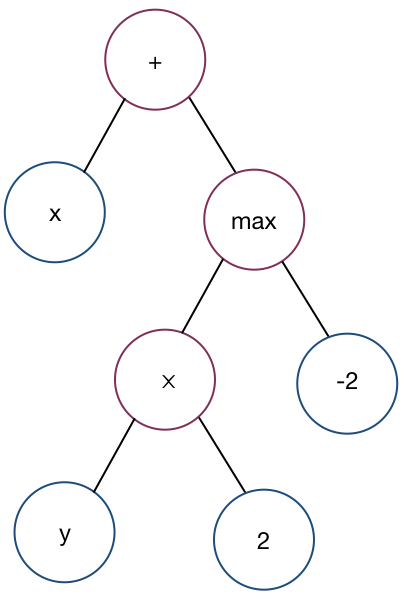
\includegraphics[width=0.3\textwidth]{pics/gp-tree.png}
	\caption{GP program that represents x + max(y $\times$ 2, -2)}
	\label{fig:gp_program}
\end{figure}


GP-based hyper-heuristics (GP-HH)  has been applied in many applications such as Job shop scheduling to evolve dispatching rules \cite{Nguyen:2014eu}. The term hyper-heuristics \cite{Cowling:2000ek} means ``heuristics to choose heuristics''.
\emph{Dispatching rule} is essentially a heuristics \cite{Panwalkar:1977fw} used in a scheduling context. 
Resource allocation problems are also in the scheduling category and they are often modeled as bin packing problems. 
GP-HH has been applied in generating heuristics for bin-packing problems \cite{Poli:2007kt,Sim:2013fe,Burke:2012gs}. These research have shown that GP-HH can generate excellent heuristics which have equal or better performance than human designed heuristics.

In the Cloud computing context,  Cloud resource allocation usually has extra constraints such as multi-dimensional resources, migration costs, heterogeneous PMs etc. These constraints make the Cloud resource allocation problem much harder than original bin packing \cite{Mann:2015ua}. Therefore, traditional bin packing approaches such as First Fit Decreasing, Best Fit etc cannot perform well in this context.  GP-HH, therefore, is a promising technique can be used to automatically generate heuristics under multiple constraints.

\subsubsection{Container-based clouds}
\paragraph{Existing approaches}
Piraghaj et al \cite{Piraghaj:2015dv} propose a framework for container-based resource management including three steps, analyzing resources to trigger migration, deciding which containers to migrate, and placing the container to a VM. In the third step, Piraghaj applies three heuristics: First-Fit, Random, and Least Full. However, this work only reports that their approach can reduce the number of VMs but does not mention how to reduce the number of PMs by migrating VMs. Therefore, this work does not consider the interactions between two levels: VM and PM. 

% \paragraph{GP-HH approach for Bilevel optimization problem}
% So far, no study has focus on using GP-HH for bilevel optimization problem. 

\section{Summary}

\bx{This chapter reviewed the main concepts of cloud resource management and server consolidation.} It also discusses the challenges of server consolidation in container-based clouds. We illustrate the limitations of existing work on three placement decision scenarios in both container-based and VM-based clouds. 

\begin{itemize}
	\item \bx{Current research lacks appropriate model to capture the relationship between containers, VMs and PMs.} Hence, most research on container-based initial placement of application conducts the placement in two independent steps: container-VM and VM-PM. These approaches neglected the interaction between two levels of placement, hence, they cannot reach a near optimal energy consumption. A bilevel model for the joint placement of containers and VMs need to be proposed. Related sub models such as energy model, workload model, variables and constraints need to be further investigated.
	\item Periodic placement of application has not been studied in the container context. A bilevel multi-objective energy model needs to be proposed which considers minimizing migration cost as well as minimizing energy consumption. 
	\item Traditional periodic placement of application mostly consider static workload. Thus, it is very likely lead to large number of adjustment of applications' placement in the future because the fluctuation of workloads. These adjustment will increase the cost for Cloud providers. In order to provide a robust placement of application, various predictable workload patterns such as linear continuously changing can be considered. It needs more investigation on how to represent various workloads and how to combine them in a compact structure.
	\item Current dynamic placement of application approaches are based on simple bin-packing algorithms and manually designed heuristics. These heuristics are either perform poorly or cannot be applied with specific constraints. A hyper-heuristic approach can learn from previous good placement patterns and automatically generate heuristics. In order to design a hyper-heuristic, features of various workload need to be investigated. 
\end{itemize}


This research aims to address the above-mentioned issues. The next chapter will focus on the initial work conducted in investigating NSGA-II for bilevel initial placement of application.


% Beloglazov and Buyya \cite{Beloglazov:2012bw} propose





% Initialization is one of the major step in resource management. It can be considered as a static problem \cite{Jennings:2015ht} or dynamic problem \cite{Beloglazov:2012bw}. 
% As we discussed in the previous section, a dynamic allocation normally cannot gives a global optimized solution of a batch of tasks. Therefore, in the context of maximizing the energy efficiency of a data center, we category initialization into a static optimization approach.

% % Previous research mainly use heuristic to solve this problem. 


% \subsection{Traditional Approaches}
% \subsection{EC Approaches}

% \section{}
% \textcolor{Maroon}{Why this field is important.}

% Cloud computing has made one critical change in software industry, it separates the role of traditional service provider into service provider and infrastructure provider. As Wei \cite{Wei:2010fn} states, ``one provides the computing of services, and the other provides the services of computing''. Therefore, this separation add one more layer between service provider and users, as: Cloud providers, Cloud users (service providers), and End users \cite{Jennings:2015ht} (see Figure \ref{fig:stakeholders}). 

% This separation of role has completely reformed the software industry \cite{Buyya:2009ix} by providing three major benefits to Cloud users. First, Cloud users do not need upfront investment in hardwares (e.g servers and networking devices) and pay for hardwares' maintenance. Second, Cloud users will not worried about the limited resources will obstruct the performance of their services when unexpected high demand occurs. The elastic nature of cloud can dynamic allocate and release resources for a service. In addition, Cloud users can pay as much as the resource usage under a \emph{pay-as-you-go} policy. Third, Cloud users can publish and update their applications at any location as long as there is an Internet connection. These advantages allow anyone or organization to deploy their softwares on Cloud in a reasonable price. 




% In this thesis, we focus on a core issue of helping Cloud providers to increase their profits. This goal can be done by two ways, attracting more Cloud users to use Cloud services and reducing the expense.








% Service models of Cloud computing are critical in solving energy consumption problem because their distinct ways of managing resources have severe effect on the problem. These distinct ways of resource management mainly result from the responsibilities among stakeholders. 

% There are three traditional service models \cite{Mell:2011jj} which describe the responsibilities among stakeholders: Infrastructure as a Service (IaaS), Platform as a Service (PaaS) and Software as a Service (SaaS). The architecture of Cloud computing is illustrate in Figure \ref{fig:architecture}.

% \begin{itemize}
% 	\item IaaS, a Cloud provider hosts hardwares such as PMs and cooling infrastructure on behalf of Cloud users. A Cloud provider also provides maintenance, management of hardware resources. 

% 	In IaaS, Cloud provider offers the fundamental resources such as CPU cores, RAMs, and network bandwidth. These resources are often encapsulated in virtualized computing units called virtual machines (VMs). Cloud providers establish a number of types of VM for simplifying the management. The `type' means a VM contains a certain quantity of resources such as 2-cores and 1 GB RAM.  \emph{Traditional} IaaS and PaaS use VM as the fundamental unit of resources.

% 	A typical procedure of a Cloud user deploying their applications in an IaaS cloud includes several steps.
% 	Initially, Cloud users estimate the resources that their applications might consume and select a type of VM which can satisfy the requirement. After Cloud users have made the decisions, they send requests to Cloud providers for a number of VMs. Finally, Cloud providers received the request, provisioned and allocated these VMs to PMs. 

% 	From the resource management perspective, the constraint in allocation of VMs is that the aggregated VMs' resources in a PM cannot exceed the capacity of the PM. After these VMs have been allocated, their types cannot be changed. During the life cycle of an application, Cloud providers can dynamically adjust the locations of VMs, provision new VMs (same type) for the replicas of an application, as well as turning on/off PMs.

	% After receiving the requests, Cloud providers choose a set of PMs and allocate the required VMs in them. Then, Cloud users can access the VMs through remote consoles. Cloud providers manage the VMs by monitoring the resource utilization of VMs and PMs. If a VM has run out of resources, an auto-scaling strategy is automatically applied to duplicate the users' VM. Finally, Cloud providers optimize the locations of VMs by consolidating them into a minimum number of PMs.


 	% \item PaaS, a Cloud provider builds a software platform on top of hardwares provided by IaaS. This platform allows a complete life-cycle of software development including development, testing and deployment.

 	% From resource management perspective, PaaS is sitting above the IaaS which means the underlying resource is still based on IaaS VM types. Different from IaaS, PaaS takes the responsibility of selecting VMs and allows Cloud users to focus on software development. 

 	% A typical procedure of a Cloud user deploying their applications in an PaaS cloud includes several steps.
 	% In the first step, Cloud users need to provide the initial estimation of the quantity of resources instead of types of VM. Then, Cloud providers determine the types of VM for applications according to the estimated resources.  After this step, resource management system conducts the provisioning and allocating as the same steps in IaaS. During the life cycle of applications, similar to IaaS, Cloud providers can also adjust the location of VMs, add new VMs, and control the status of PMs. Different from IaaS, Cloud providers can change the type of VM for an application according to it needs.

 	% The system monitors the utilization of a number of PM and VM and through adjustment of their location to optimize the energy consumption of the data center. The input is a list of VMs (e.g CPU cores and RAMs) and a list of PMs. The task is to put the VMs into these PMs so that the VMs only use a minimum number of PMs. The sizes of VMs and PMs are fixed. A system can only adjust which VM is allocated to which PM. A general constraint is the sum of resources of the VMs inside a PM cannot exceed the capacity of the PM.

 	% \item SaaS describes the relationship between Cloud users and End users. End users create workloads for applications. Although this service model does not directly related to the resource management, it provides the fundamental reasons for resource management and optimization. Because of the dynamic nature of workloads, the underlying resources must also be dynamic adjusted to meet the requirement.
% \end{itemize}



% \textcolor{Maroon}{Describe the current ``hot topics'' in the field}

% \subsection{Research Fields in Cloud Computing}
% Cloud computing paradigm has been applied for over ten years, however, many problems have been fully addressed and new challenges has emerged along with new technologies. We summarize some of the hot research fields.

% \subsubsection{Automated service provisioning}
% The key functionality of Cloud computing is to provide an elastic resource management for applications. Cloud users desire a complete automated service provisioning which automatically allocate and release resources for applications that satisfies the service level objective (SLOs). 

% Current automated service provisioning normally involves three steps \cite{Zhang:2010vo}: 
% (1) Constructing a performance model which can predict the need of resources of a given application. (2) Periodically predict the future resource requirement of the application using the model. (3) Automatically allocating resources to the application.

% There are multiple difficulties in this problem. First problem is the mapping between SLOs such as Quality of Service (QoS) requirements: throughput, response time and etc, to low level hardwares such as CPU and memory requirements. This problem is often addressed as Resource Demand Profiling. Approaches are categorized into model-driven, where a predefined model is used to identify the resources' requirement of applications; or statistical techniques which use machine learning algorithms to predict the requirement in the future.

% In the model-driven category, Urgaonkar and et al \cite{Urgaonkar:2005uo} that use a queuing model to determine the resources (each server as the resource unit) for multi-tier application. They model each server as as a G/G/1 queuing system; Bennani and Menasce \cite{Bennani:2005wd} also propose a multiclass queuing network models for both online transactions applications and batch processing applications. 

% In statistical approaches, Li and et al \cite{Li:2011cx} develop a trace-and-replay tool called CloudProphet to predict a legacy application's performance. It monitors the performance of the application locally and replays the workload in the cloud for prediction. Gong and et al. \cite{Gong:2010td} use a signal processing algorithm - Fast Fourier Transform to detect 
% repeating resource usage patterns, and a statistical learning algorithm - discrete-time Markov chain to build short-term demand predictions.

% Furthermore, the decisions are often made in an on-line fashion to trigger the allocation and de-allocation of resources in order to satisfy the fluctuate workload over multiple time scales \cite{Crovella:1997tr}. 



% \subsubsection{Virtual machine migration}
% \subsubsection{Server consolidation}
% \subsubsection{Energy management}
% \subsubsection{Novel cloud architectures}

% \subsection{Container as a Service}
% Our proposed optimization approaches are based on a new service model: 

% Before explaining the details of resource management strategies, we first illustrate several characteristics of resource management in IaaS.
% Firstly, we illustrate the disadvantages of traditional IaaS and PaaS and discuss the reasons of why current approaches cannot completely overcome these problems. From there, we explain why CaaS is a prescription of their problems.




% Specifically, the profit can be improved by reducing the energy consumption. A direct way to reduce energy consumption is to always use a minimum number of Physical machines (PMs) hosting applications. This is because the more PMs are running, the more energy they are 
% consumed.



% Cloud computing is derived from a few computing paradigms including Grid computing, service computing and etc. Grid computing allow their users to run a large-scale computational intensive tasks on a geographically distributed computing resources. Cloud computing is similar to grid computing of utilizing a group distributed
% comtpuing resources. Unlike grid takes each computer as an individual resource, Cloud computing virtualizes the Physical resources into VMs and provides a centralized resource management. Service computing, including Service Oriented Architecture (SOA) and Web services, focus on constructing large scale Web-based application using the Internet. In SOA, web services are the building blocks of softwares and they can be distributed developed, deployed and composited through the Internet. The technologies, such as SOAP and REST, enables Web serivces.










% Service computing such as Service Oriented Architecture and Web Services, focus on the seamless business processes. 

% The purpose of Cloud computing is to reduce the cost of ``in-house'' 




% The separate responsibility between Cloud providers and Cloud users has completely reformed the software industry \cite{Buyya:2009ix} by providing three major benefits to Cloud users.
% First, Cloud users do not need upfront investment in hardwares (e.g PMs and networking devices) and pay for hardwares' maintenance. Therefore, it eliminates the risk of initial investment.
% Second, Cloud users do not need to worry about the limited resources which can obstruct the performance of their services when unexpected high demand occurs. Cloud providers off an elastic nature of Cloud which can dynamic allocates and releases resources for a software.  Cloud users only need to pay the resources that they have used under a \emph{pay-as-you-go} policy. Third, Cloud users can publish and update their applications at any location as long as there is an Internet connection. These advantages allow anyone or organization to deploy their softwares on Cloud in a reasonable price. 

% As previous section mentioned, our goal in this thesis is to help Cloud providers to increase their profit from data centers. Specifically, we focus on how to save money by cutting expenses of Cloud data centers. 
% Cloud providers have two ways of achieving this goals, one is to provide better Quality of Service (QoS) service such as high throughput, low latency, and high availability, to attract more Cloud users to use Cloud services. The other way is to save money 
% Each stakeholder has their objectives.  End users consume application. They require a guarantee quality of softwares including functional requirements which are the functionalities defined by Cloud users, and non-functional requirements such as availability, security, and network latency. Cloud users develop and deploy softwares on Cloud. They provide functional correct softwares and they also desire the non-functional requirements of softwares can be satisfied by Cloud resources. Cloud providers offer low-level resources such as computational power, storage and network bandwidth. Cloud providers want to increase their profit by attracting more Cloud users to use Cloud services and reducing the expense caused
% \begin{figure}[H]
% 	\centering
% 	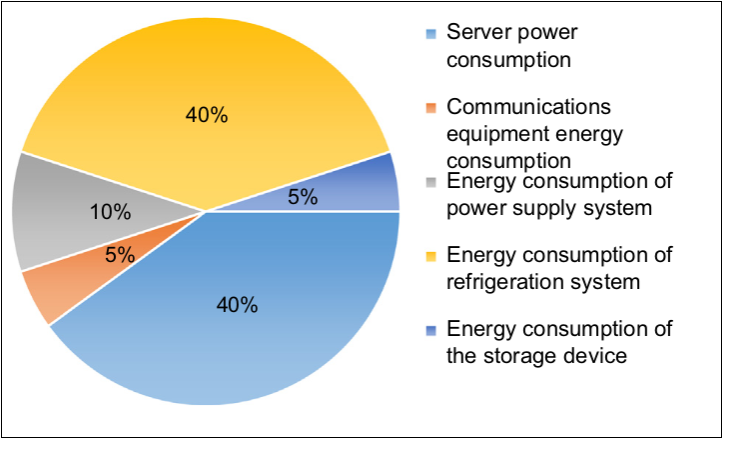
\includegraphics[width=0.5\textwidth]{pics/energyConsumption.png}
% 	\caption{Energy consumption distribution of data centers \cite{Rong:2016js}}
% 	\label{fig:consumption}
% \end{figure} 








% \subsection{Resource Management in IaaS}
% The resource management in IaaS can be roughly separated into three \cite{Svard:2015ic, Mishra:2012kx} which are applied in different scenarios: Application initialization, Prediction and Global consolidation, and Dynamic resource management (see Figure \ref{fig:management}). 

% \begin{figure}
% 	\centering
% 	\begin{subfigure}[b]{0.9\textwidth}
% 		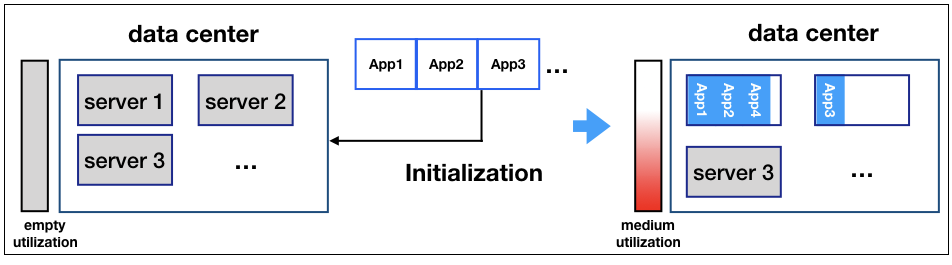
\includegraphics[width=\textwidth]{pics/initialization.png}
% 		\caption{Initialization}
% 	\end{subfigure}
% 	\begin{subfigure}[b]{0.9\textwidth}
% 		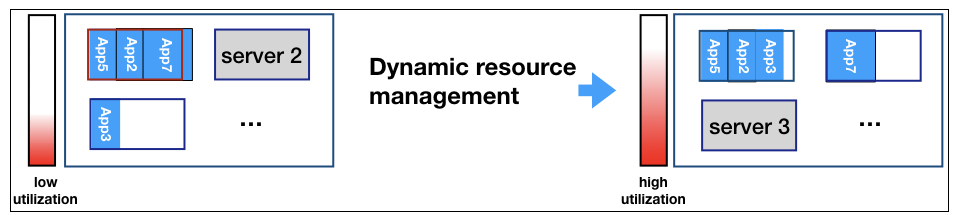
\includegraphics[width=\textwidth]{pics/dynamic_resource.png}
% 	\caption{Dynamic resource management}
% 	\end{subfigure}
% 	\begin{subfigure}[b]{0.9\textwidth}
% 		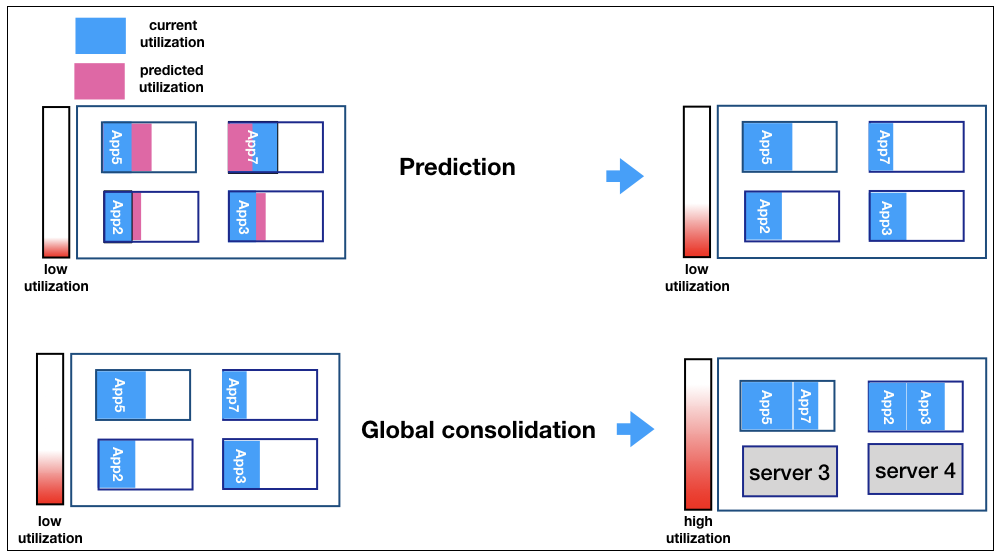
\includegraphics[width=\textwidth]{pics/predict_consolidate.png}
% 	\caption{Prediction and Consolidation}
% 	\end{subfigure}
% 	\caption{Three stages of resource management in IaaS}
% 	\label{fig:management}
% \end{figure}


% Server consolidation is the core functionality involving in all Cloud resource management operations. These operations

% Data center constantly receives new requests for applications initialization. Once the new applications have been allocated, the utilization begins to drop. This is because, initially, applications are compactly allocated on PMs. As old applications instance are released because of canceling, the compact structure become loose. Dynamic resource management is a process which can slow the utilization from decreasing. It consolidates by re-allocating one application at a time. Finally, global consolidation is conducted periodically to dramatically improve the resource utilization.
% \begin{enumerate}
% 	\item \emph{Application initialization} is applied when new applications or new VMs arrive and the problem is to allocate them into a minimum number of PMs.

% 	In this problem, a set of applications or VMs are waiting in a queue. The resource capacity of the PM and usage by applications are characterized by a vector of resource utilizations including CPU, memory and etc. Then, the allocation system must select a minimum number of PMs to accommodate them so that after the allocation, the resource utilizations remain high. The problem is to consider the different combinations of applications so that the overall resource utilization is high. This problem is naturally modeled as a static bin-packing problem \cite{CoffmanJr:1996ui} which is a NP-hard problem meaning it is unlikely to find an optimal solution of a large problem. 

% 	\item \emph{Prediction and Global consolidation} is conducted periodically to adjust the current allocation of applications so that the overall utilization is improved.

% 	In this problem, time is discrete and it can be split into basic time frames, for example: ten seconds. A periodical operation is conducted in every $N$ time frames.
% 	A cloud data center has a highly dynamic environment with continuous arriving and releasing of applications. Releasing applications cause hollow in PMs; new arrivals cannot change the structure of current allocation. Therefore, after the initial allocation, the overall energy efficiency is likely to drop along with time elapsing. 

% 	In prediction, an optimization system takes  the current applications' utilization records as the input. Make a prediction of their utilization in the next period of time. 
% 	In Global consolidation, based on the predict utilization and the current allocation - including a list of applications/VMs and a list of PMs, the system adjusts the allocation so that the global resource utilization is improved.

% 	In comparison with initialization, instead of new arrivals, the global consolidation considers the previous allocation. Another major difference is that global consolidation needs to minimize the differences of allocation before and after the optimization. This is because the adjustment of allocation relies on a technique called live migration \cite{Clark:2005uda}, and it is a very expensive operation because it occupies the resources in both the host and the target. Therefore, global optimization must be considered as a time-dependent activity which makes the optimization even difficult.

% In comparison with dynamic consolidation, global consolidation takes a set of VMs as input instead of one. Therefore, it is time consuming and often treated as a static problem.
% 	\item \emph{Dynamic resource management} 
%  	Dynamic resource management is applied in three scenarios. \textbf{First},  it is applied when a PM is overloading. In order to prevent the QoS from dropping, an application is migrated to another PM. This is called hot-spot mitigation \cite{Mishra:2012kx}. \textbf{Second}, it is applied when a PM is under-loading. Under-loading is when a PM is in a low utilization state normally defined by a threshold. At this moment, all the applications in the under-loading PM are migrated to other active PMs, so the PM becomes empty and can be turned off. This is called dynamic consolidation. \textbf{Third}, it is applied when a PM having very high level of utilization while others having low. An adjustment is to migrate one or more application from high utilized PMs to low ones. This is called load balancing.

% 	No matter which scenario it is, a dynamic resource management always involves three steps . 
% 	\begin{itemize}
% 		\item \emph{When to migrate?} refers to determine the time point that a PM is overloaded or underloaded. It is often decide by a threshold of utilization.
% 		\item \emph{Which application to migrate?} refers to determine which application need to be migrated so that it optimize the global energy consumption.
% 		\item \emph{Where to migrate?} refers to determine which host that an application is migrated to. This step is called dynamic placement of application which is directly related to the consolidation, therefore, it is decisive in improving energy-efficiency. 
% 	\end{itemize}

% 	Among three operations, dynamic placement of application is a dynamic and on-line problem.
% 	The term ``dynamic'' means the request comes at an arbitrary time point. An on-line problem is a problem which has on-line input and requires on-line output \cite{Borodin:uQcy_H6C}. It is applied when a control system does not have the complete knowledge of future events.

% 	There are two difficulties in this operation, firstly, dynamic placement of application requires a fast decision while the search space is very large (e.g hundreds of thousands of PMs). Secondly, migrate one application at a time is hard to reach a global optimized state.

% \end{enumerate}



% Finally, a consolidation plan includes four major items:
% 			\begin{enumerate}
% 				\item A list of existing PMs after consolidation
% 				\item A list of new virtual machines created after consolidation
% 				\item A list of old PMs to be turned off after consolidation
% 				\item The exact placement of applications and services
% 			\end{enumerate}

% By the nature of Cloud resource management, server consolidation techniques can also be categories into static and dynamic methods. Static method is a time consuming process which is often conducted off-line in a periodical fashion; initialization and global consolidation belong to this category. It provides a global optimization to the data center. Dynamic method adjusts PMs in real time. It often allocates one application at a time. Therefore, it can be executed quickly and often provides a local optimization to the data center.


















% They are bonded by the Quality of service and computing resource. Quality of service and the computing resources are the two sides of a coin. 



% Cloud users deploy their software on Clouds. They want to increase the profit by increasing income and decreasing expense. In order to accomplish this goal, they can attract more End suers by improving the functionality of softwares and the non-functionality features by guaranteeing Quality of Service (QoS). To improve the non-functionality features, Cloud users need to reserve enough resources as well as minimizing the resource so that the cost is low.


% service capacity planning is the core process. The capacity planning has two conflicting objectives, on one hand, it must meet End users' QoS requirement by using enough resources.  On the other hand, the cost must be minimized. In pre-Cloud era, the capacity planning determines the upfront investment in infrastructure, therefore, capacity, reliability, and scalability are all need to be carefully considered and balanced. In Cloud environment, the burden of capacity planning is largely released by elastic resource management and the pay-as-you-go policy.


% Cloud users identify a list of critical QoS parameters called Service Level Agreement (SLA) which specifies the non-functional requirements such as throughput, latency, and availability. These QoS parameters are mapped to resources (e.g. CPU, memory, network bandwidth) which can satisfy these requirements. Violation of SLA will lead to penalty and decreasing in number of users. Therefore, in essence, the key to attract more users is an effective resource management system which can rapidly react to the fluctuating resource demand. 

% Beside increase the income, reduce the expense is another way to improve profit. As previous section mentioned, energy consumption is the main source of expense. In energy consumption, server energy consumption is the core that needs to be improved. 

% \subsection{Energy-aware Resource Management}
% \subsection{An Overview of Evolutionary Computation}


% In order to understand Cloud computing, firstly we will illustrate the five essential elements of Cloud computing and their advantages.

% Cloud computing has five essential elements:


% \textcolor{Blue}{What is your purpose to describe the following content?}
% \textcolor{Red}{
% 	I would like to discuss the differences, advantages of disadvantage of the resource management in different service models. Therefore, after illustrate how they are work. The point is to compare the resource management. And then, lead to a new service model. And the advantage of new service model should be obvious. 
% }\\
% Traditional Cloud computing has three service model as illustrated in Figure \ref{}.
% Infrastructure as a Service (IaaS), Platform as a Service (PaaS), and Software as a Service. 
% \subsection{Resource Management}
% Scope of Cloud computing resource management.
% \begin{enumerate}
%  \item Actors
%  \item Management Objectives
%  \item Resource Types
%  \item Enabling Technologies
% \end{enumerate}






